\documentclass[oneside,openany,a4paper,12pt]{article}

% بسته‌های ریاضی و عمومی مورد نیاز
\usepackage{amsthm,amssymb,amsmath}
\usepackage[top=30mm, bottom=25mm, left=25mm, right=30mm]{geometry}
\usepackage{graphicx}
\usepackage{framed}
\usepackage{fancyhdr}
\usepackage{setspace}
\usepackage{multirow}
\usepackage{float}
\usepackage{subfigure}
\usepackage{booktabs}

% بسته‌ و دستوراتی برای ایجاد لینک‌های رنگی
\usepackage[pagebackref=false,colorlinks,linkcolor=blue,citecolor=blue]{hyperref}

% فراخوانی بسته زی‌پرشین و تعریف قلم‌های فارسی و انگلیسی
\usepackage{xepersian}
\settextfont[Path=font/,Extension=.ttf,Scale=1.1,
    BoldFont=XB NiloofarBd,
    ItalicFont=XB NiloofarIt,
    BoldItalicFont=XB NiloofarBdIt
]{XB Niloofar}
\setlatintextfont[Scale=0.9]{Times New Roman}
\setdigitfont[Path=font/,Extension=.ttf,Scale=1.1,
    BoldFont=XB NiloofarBd,
    ItalicFont=XB NiloofarIt,
    BoldItalicFont=XB NiloofarBdIt
]{XB Niloofar}

\makeatletter
\providecommand{\AutoPersianDigits}{}
\makeatother

\begin{document}
\AutoPersianDigits
\setstretch{1.4}

\begin{center}
    \vspace*{1cm}
    \Huge\textbf{گزارش تفصیلی شبیه‌ساز مأموریت پهپاد \lr{(DARTSim)} و یکپارچه‌سازی روش \lr{RS-DRL} با حلقه \lr{MAPE-K}}
\end{center}

\newpage
\tableofcontents
\newpage

\section{مقدمه و معرفی بستر شبیه‌سازی DARTSim}
شبیه‌ساز مأموریت تاکتیکی پهپادها \lr{(DARTSim -- Dynamic Airspace Real-Time Simulation)} \cite{MorenoDART2019} یک بستر شبیه‌سازی هوایی فیزیکی-سایبری جامع برای ارزیابی و تحلیل تصمیم‌گیری‌های انطباقی زمان اجرای تیم‌های پهپادی در محیط‌های پرخطر و متخاصم است. در این سیستم، تیمی از پهپادها مأموریت پیمایش و شناسایی را در یک حریم هوایی متخاصم اجرا می‌کنند و باید با اتخاذ تصمیمات تاکتیکی و وفقی، بقای خود را حفظ کرده و در عین حال، اهداف مأموریت را بیشینه نمایند.

ریشه اصلی این شبیه‌ساز در مسئله تیم پهپادهای خودگردان \lr{(UAV Team)} است که نخستین‌بار توسط مورنو و همکاران \cite{moreno2015proactive} به عنوان یک محک استاندارد برای سیستم‌های خودوفق تحت عدم قطعیت معرفی گردید. این بستر چالش‌های بسیار متفاوتی را نسبت به سایر سیستم‌ها (نظیر شبکه‌های حسگر بی‌سیم DeltaIoT) ارائه می‌دهد؛ زیرا تصمیم‌گیری‌ها باید به صورت بلادرنگ در فضای حالت پیوسته و فضای اقدام گسسته اتخاذ شوند.

یکی از جنبه‌های کلیدی در این مأموریت، مصالحه محوری ارتفاع \lr{(Altitude Trade-off)} است:
\begin{itemize}
    \item \textbf{پرواز در ارتفاع پایین:} احتمال شناسایی اهداف زمینی توسط حسگرهای پهپاد را افزایش می‌دهد، اما در مقابل، پهپادها را در معرض رادارهای دفاعی و تهدیدهای زمینی دشمن قرار داده و ریسک انهدام را به شدت بالا می‌برد.
    \item \textbf{پرواز در ارتفاع بالا:} ریسک شناسایی پهپادها توسط تهدیدات زمینی و انهدام آن‌ها را به حداقل می‌رساند، اما به دلیل افزایش فاصله، کیفیت قرائت حسگرهای پهپاد افت کرده و شناسایی اهداف زمینی را با چالش جدی مواجه می‌سازد.
\end{itemize}

نمودار مفهومی عوامل تاثیرگذار بر اهداف وابستگی‌پذیری تیم پهپادی در شکل \ref{fig:dartsim_system_diagram} نشان داده شده است. این شکل نشان می‌دهد که چگونه عوامل پیکربندی (قابل‌کنترل) و عوامل محیطی (غیرقابل‌کنترل) در دل یک محیط متخاصم بر روی اهداف شناسایی هدف و اجتناب از تهدید اثر می‌گذارند.

\begin{figure}[H]
  \centering
  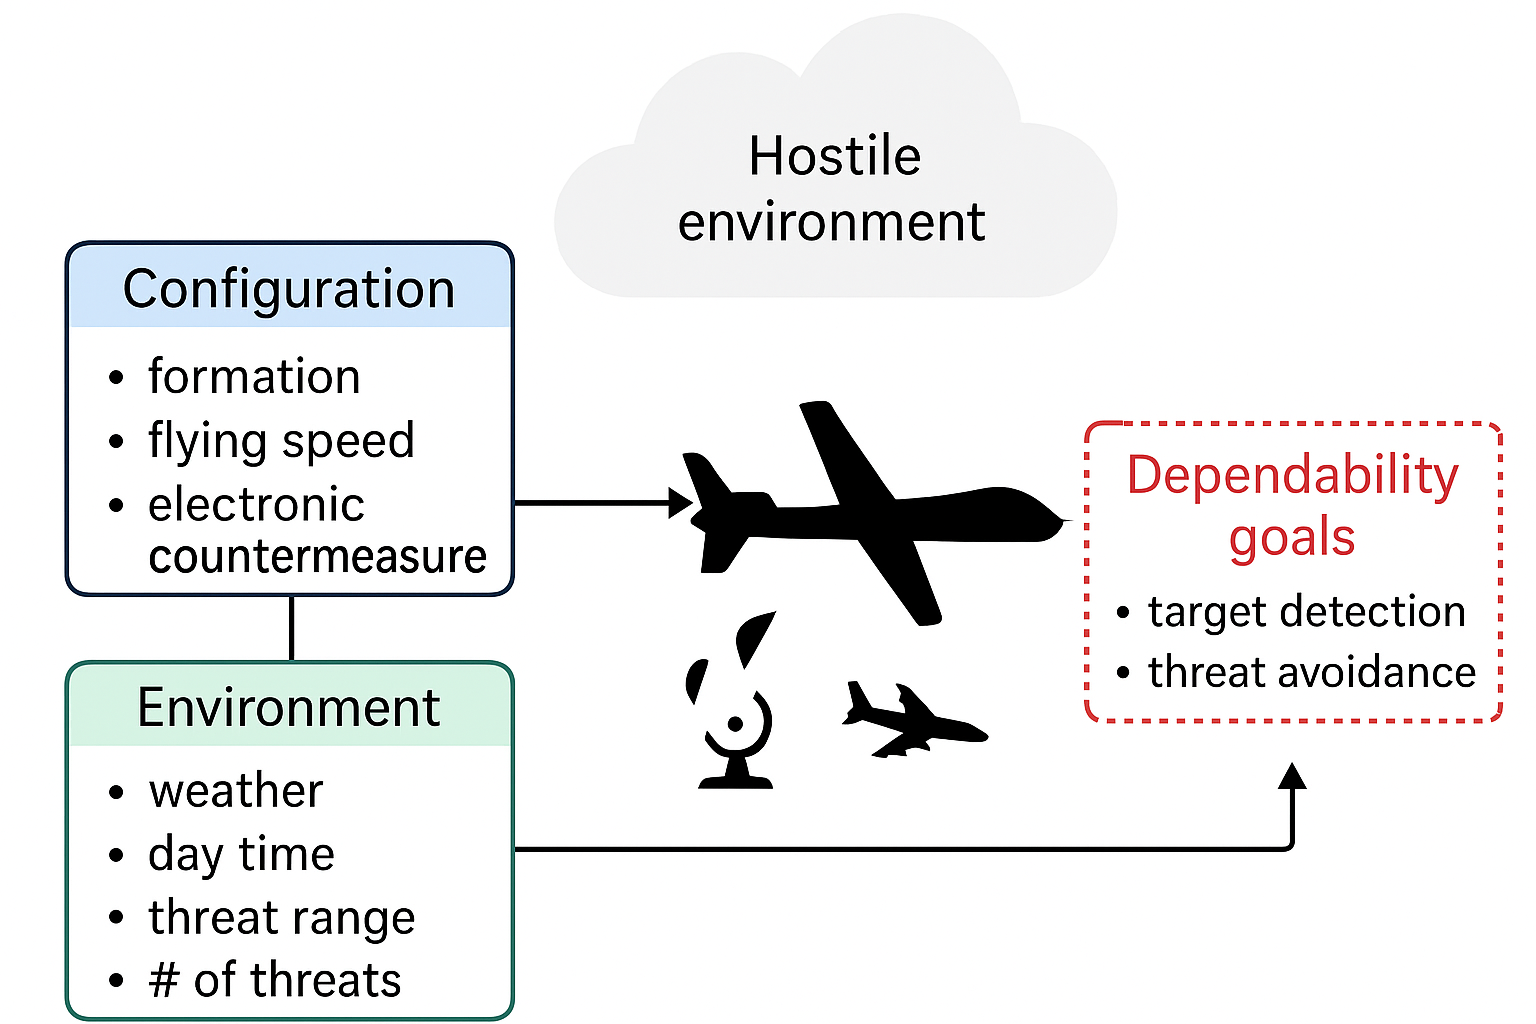
\includegraphics[width=0.85\textwidth]{figures/dartsim_system_diagram.png}
  \caption{نمودار مفهومی عوامل اثرگذار بر اهداف وابستگی‌پذیری تیم پهپادی DARTSim}
  \label{fig:dartsim_system_diagram}
\end{figure}

\section{فضای معنایی و الزامات سیستم}

\subsection{فضای معنایی (\lr{Semantic Space})}
رفتار سیستم پهپادی توسط مجموعه‌ای از عوامل پیکربندی و عوامل محیطی تعیین می‌شود که مجموعاً «فضای معنایی» سیستم را تشکیل می‌دهند. این عوامل در جدول \ref{tab:dartsim_semantic_space} خلاصه شده‌اند:

\begin{table}[H]
\centering
\caption{فضای معنایی سیستم پهپادی DARTSim}
\label{tab:dartsim_semantic_space}
\resizebox{\textwidth}{!}{%
\begin{tabular}{llll}
\hline
\textbf{عامل} & \textbf{نوع} & \textbf{دامنه/بازه} & \textbf{توضیح} \\ \hline
\lr{formation} & پیکربندی (کنترلی) & \lr{\{tight, loose\}} & آرایش هندسی تیم پهپادها حین مأموریت \\
\lr{flying speed} & پیکربندی (کنترلی) & \lr{[5, 50] mph} & سرعت پرواز پهپادها (تاثیرگذار بر سرعت و دقت سنسورها) \\
\lr{ECM} & پیکربندی (کنترلی) & \lr{\{ON, OFF\}} & فعال‌سازی اخلال‌گر الکترونیکی برای مقابله با رادارهای فعال \\
\lr{weather} & محیطی (عدم قطعیت) & \lr{\{sun, clouds, rain, fog\}} & وضعیت آب و هوایی تاثیرگذار بر نویز حسگرها \\
\lr{day time} & محیطی (عدم قطعیت) & شبانه روز (ساعت) & زمان پرواز که بر روشنایی و سنسورها اثر می‌گذارد \\
\lr{threat range} & محیطی (عدم قطعیت) & \lr{[0.9, 3.7] km} & شعاع و برد راداری تهدیدهای پدافندی دشمن \\
\lr{\# threats} & محیطی (عدم قطعیت) & عدد صحیح \lr{[1, 10]} & تعداد تهدیدهای فعال مستقر در نقشه مأموریت \\ \hline
\end{tabular}%
}
\end{table}

\subsection{الزامات و اهداف مأموریت}
اهداف مأموریت در شبیه‌ساز DARTSim از دو الگوی اصلی و پارامتری الزامات مشتق می‌شوند که حول مفهوم محوری مصالحه ارتفاع شکل گرفته‌اند:
\begin{enumerate}
    \item \textbf{الگوی شناسایی هدف ($\Phi_0$):} «هنگامی‌که ارتفاع پهپادها بین $\theta_1$ و $\theta_2$ متر است، تیم پهپادی باید در بیش از $p_1$ درصد موارد اهداف زمینی را شناسایی کند.» هدف این الزام، بیشینه‌سازی قابلیت اطمینان مأموریت است.
    \item \textbf{الگوی اجتناب از تهدید ($\Phi_1$):} «هنگامی‌که ارتفاع پهپادها بین $\theta_1$ و $\theta_2$ متر است، تهدیدات موجود باید در کمتر از $p_2$ درصد موارد پهپادها را شناسایی کنند.» هدف این الزام، بیشینه‌سازی امنیت و نرخ بقای تیم است.
\end{enumerate}

با نمونه‌سازی این الگوها بر روی شش بازه ارتفاعی مختلف و آستانه‌های احتمال متناظر، در مجموع ۱۲ الزام ملموس (۶ مورد شناسایی و ۶ مورد اجتناب) تعریف می‌شود. مقادیر دقیق پارامتری این ۱۲ الزام در جدول \ref{tab:dartsim_requirements_instantiation} خلاصه شده است:

\begin{table}[H]
\centering
\caption{نمونه‌سازی ۱۲ الزام ملموس مأموریت پهپاد بر اساس بازه‌های ارتفاعی و آستانه‌های احتمال}
\label{tab:dartsim_requirements_instantiation}
\resizebox{\textwidth}{!}{%
\begin{tabular}{ccccc}
\hline
\textbf{الزام} & \textbf{الگوی مرجع} & \textbf{بازه ارتفاعی $[\theta_1, \theta_2]$ (متر)} & \textbf{نوع معیار} & \textbf{آستانه احتمال ($p_1$ یا $p_2$)} \\ \hline
$Req_1$ & $\Phi_0$ (شناسایی) & $[0, 100]$ & بیشینه کردن شناسایی & $p_1 > 0.90$ \\
$Req_2$ & $\Phi_0$ (شناسایی) & $[100, 200]$ & بیشینه کردن شناسایی & $p_1 > 0.85$ \\
$Req_3$ & $\Phi_0$ (شناسایی) & $[200, 300]$ & بیشینه کردن شناسایی & $p_1 > 0.75$ \\
$Req_4$ & $\Phi_0$ (شناسایی) & $[300, 400]$ & بیشینه کردن شناسایی & $p_1 > 0.65$ \\
$Req_5$ & $\Phi_0$ (شناسایی) & $[400, 500]$ & بیشینه کردن شناسایی & $p_1 > 0.55$ \\
$Req_6$ & $\Phi_0$ (شناسایی) & $[500, 600]$ & بیشینه کردن شناسایی & $p_1 > 0.50$ \\ \hline
$Req_7$ & $\Phi_1$ (اجتناب) & $[0, 100]$ & کمینه کردن شناسایی رادار & $p_2 < 0.60$ \\
$Req_8$ & $\Phi_1$ (اجتناب) & $[100, 200]$ & کمینه کردن شناسایی رادار & $p_2 < 0.50$ \\
$Req_9$ & $\Phi_1$ (اجتناب) & $[200, 300]$ & کمینه کردن شناسایی رادار & $p_2 < 0.35$ \\
$Req_{10}$ & $\Phi_1$ (اجتناب) & $[300, 400]$ & کمینه کردن شناسایی رادار & $p_2 < 0.20$ \\
$Req_{11}$ & $\Phi_1$ (اجتناب) & $[400, 500]$ & کمینه کردن شناسایی رادار & $p_2 < 0.10$ \\
$Req_{12}$ & $\Phi_1$ (اجتناب) & $[500, 600]$ & کمینه کردن شناسایی رادار & $p_2 < 0.05$ \\ \hline
\end{tabular}%
}
\end{table}

شایان ذکر است که در فرمول‌بندی یادگیری تقویتی پیشنهادی رساله، به دلیل عدم دسترسی به مدل وارسی صوری زمان اجرا، این ۱۲ الزام به صورت یک تابع پاداش چندهدفه تجمیعی (فرمولاسیون بخش بعد) پاداش‌دهی می‌شوند. با این حال، حلقه خودمختار MAPE-K در زمان اجرا چهار آستانه کیفی کلان را به عنوان سنجه‌های رضایت‌بخش پایش می‌کند: حداقل پاداش اپیزودیک $0.7$، حداقل نرخ موفقیت مأموریت $80\%$ (در بازه ۱۰ اپیزود اخیر)، حداکثر زمان تصمیم‌گیری $1000$ میلی‌ثانیه، و حداقل کسر اهداف شناسایی‌شده $60\%$.


\section{معماری و فرمول‌بندی مسئله به عنوان فرآیند تصمیم‌گیری مارکوف (\lr{MDP})}
برای اعمال روش یادگیری تقویتی عمیق بر روی DARTSim، این سیستم در قالب یک فرآیند تصمیم‌گیری مارکوف استاندارد ($\mathcal{M} = (S, A, P, R, \gamma)$) فرمول‌بندی می‌شود:

\subsection{فضای حالت ($S$)}
حالت جاری سیستم در هر گام زمانی به صورت یک بردار ۱۷ بعدی ($s_t \in \mathbb{R}^{17}$) مدل‌سازی می‌شود که شامل متغیرهای زیر است:
\begin{itemize}
    \item \textbf{موقعیت مکانی ($2$ بعد):} مختصات نرمال‌شده پهپادها ($X, Y$) نسبت به ابعاد نقشه.
    \item \textbf{جهت حرکت ($2$ بعد):} بردار جهت حرکت نرمال‌شده پهپادها.
    \item \textbf{پیکربندی جاری ($5$ بعد):} ارتفاع جاری (نرمال‌شده)، وضعیت آرایش تیمی (\lr{TIGHT} به عنوان \lr{1.0} و \lr{LOOSE} به عنوان \lr{0.0})، وضعیت فعال‌بودن اخلال‌گر الکترونیکی \lr{ECM} (روشن به عنوان \lr{1.0} و خاموش به عنوان \lr{0.0})، زمان باقی‌مانده تا اتمام افزایش ارتفاع \lr{(TTC IncAlt)}، و زمان باقی‌مانده تا اتمام کاهش ارتفاع \lr{(TTC DecAlt)}.
    \item \textbf{قرائت حسگر تهدید ($5$ بعد):} یک بردار باینری ۵ تایی که وجود یا عدم وجود تهدید را در ۵ سلول پیشِ‌رو نشان می‌دهد.
    \item \textbf{قرائت حسگر هدف ($5$ بعد):} یک بردار باینری ۵ تایی که وجود یا عدم وجود اهداف زمینی را در ۵ سلول پیشِ‌رو نشان می‌دهد.
\end{itemize}

\subsection{فضای اقدام ($A$)}
فضای اقدام شامل ۸ اقدام تاکتیکی گسسته است که سیستم خودوفق می‌تواند برای تطبیق پهپادها اتخاذ کند:
\begin{itemize}
    \item اقدام ۰ \lr{(IncAlt)}: افزایش ارتفاع به میزان ۱ سطح.
    \item اقدام ۱ \lr{(DecAlt)}: کاهش ارتفاع به میزان ۱ سطح.
    \item اقدام ۲ \lr{(IncAlt2)}: افزایش شدید ارتفاع به میزان ۲ سطح.
    \item اقدام ۳ \lr{(DecAlt2)}: کاهش شدید ارتفاع به میزان ۲ سطح.
    \item اقدام ۴ \lr{(GoTight)}: فشرده‌سازی آرایش هندسی تیمی.
    \item اقدام ۵ \lr{(GoLoose)}: باز کردن و افزایش فاصله در آرایش تیمی.
    \item اقدام ۶ \lr{(EcmOn)}: روشن کردن سیستم جنگ الکترونیک ECM.
    \item اقدام ۷ \lr{(EcmOff)}: خاموش کردن سیستم جنگ الکترونیک ECM.
\end{itemize}

\subsection{تابع پاداش چندهدفه ($R$)}
پاداش به دست آمده به صورت ترکیب وزنی و چندهدفه بر پایه پاداش‌های تنک \lr{(Sparse)} فرمول‌بندی شده است. در طول مأموریت (گام‌های میانی)، یک جریمه گام ناچیز ($c_{\text{step}} = -0.01$) به جهت تشویق پهپاد به حرکت سریع‌تر اعمال می‌شود. پاداش اصلی در پایان مأموریت (گام پایانی) بر اساس معیارهای زیر محاسبه می‌گردد:
\begin{equation}
R(s_t, a_t) = w_{\text{success}} \cdot r_{\text{success}} + w_{\text{targets}} \cdot r_{\text{targets\_detected}} + w_{\text{survival}} \cdot r_{\text{survival}} + w_{\text{efficiency}} \cdot r_{\text{efficiency}}
\end{equation}
که در آن وزن‌های پیش‌فرض برابرند با:
\begin{itemize}
    \item $w_{\text{success}} = 0.4$: پاداش موفقیت کامل مأموریت (رسیدن به انتهای مسیر).
    \item $w_{\text{targets}} = 0.3$: کسر اهداف شناسایی‌شده نسبت به کل اهداف نقشه.
    \item $w_{\text{survival}} = 0.2$: بقای تیم پهپادی (در صورت انهدام جریمه سنگین $w_{\text{destruction}} = -0.5$ اعمال می‌شود).
    \item $w_{\text{efficiency}} = 0.1$: میانگین زمان تصمیم‌گیری (پاداش بیشتر برای تصمیمات سریع‌تر).
\end{itemize}

تعاریف عملیاتی و فرمول‌های دقیق معیارهای فوق به شرح زیر است:
\begin{itemize}
    \item \textbf{موفقیت مأموریت \lr{(Mission Success)}:} رسیدن ایمن پهپادها به انتهای طول افقی حریم هوایی نقشه بدون منفجر شدن در محدوده گام‌های مجاز زمانی ($t_{\text{max}} = 100$). در صورت موفقیت، $r_{\text{success}} = 1.0$ و در غیر این صورت $r_{\text{success}} = 0.0$ است.
    \item \textbf{نرخ شناسایی اهداف \lr{(Target Detection Rate)}:} کسر تعداد اهداف شناسایی‌شده توسط سنسورهای هوابرد پهپاد نسبت به کل اهداف فیزیکی مستقر در سطح نقشه، یعنی:
    \begin{equation}
    r_{\text{targets\_detected}} = \frac{N_{\text{detected}}}{N_{\text{total\_targets}}}
    \end{equation}
    \item \textbf{نرخ بقا \lr{(Survival Rate)}:} یک متغیر باینری که نشان‌دهنده زنده‌ماندن پهپاد تا پایان مسیر است. در صورت انهدام توسط پدافند هوایی، $r_{\text{survival}} = 0.0$ و جریمه انهدام اعمال می‌شود، در غیر این صورت $r_{\text{survival}} = 1.0$ است.
    \item \textbf{بهره‌وری زمانی \lr{(Time Efficiency)}:} برای مأموریت‌های موفق، متناسب با زمان صرف‌شده نسبت به حداکثر گام‌ها محاسبه می‌شود:
    \begin{equation}
    r_{\text{efficiency}} = 1 - \frac{t_{\text{steps}}}{t_{\text{max}}}
    \end{equation}
\end{itemize}

\subsection{تنظیم ابرپارامترها و اعتبارسنجی مدل}
به منظور آموزش مدل‌های یادگیری تقویتی پیشنهادی \lr{(RS-DRL)} و DQN پایه، تنظیم دقیق ابرپارامترها از اهمیت بالایی برخوردار است. انتخاب ابرپارامترها با استفاده از جستجوی شبکه‌ای \lr{(Grid Search)} روی داده‌های اعتبارسنجی مستقل انجام شده است. جدول \ref{tab:hyperparameters} مقادیر بهینه انتخاب‌شده برای پارامترهای مختلف آموزش را نشان می‌دهد.

\begin{table}[H]
\centering
\caption{ابرپارامترهای بهینه تنظیم‌شده برای فرآیند آموزش مدل}
\label{tab:hyperparameters}
\begin{tabular}{lc}
\hline
\textbf{ابرپارامتر} & \textbf{مقدار بهینه} \\ \hline
نرخ یادگیری \lr{(Learning Rate)} & $10^{-4}$ \\
ضریب تنزیل \lr{(Discount Factor $\gamma$)} & $0.99$ \\
اندازه مینی‌بچ \lr{(Batch Size)} & $32$ \\
ظرفیت بافر بازپخش \lr{(Replay Buffer Capacity)} & $50{,}000$ \\
فرکانس به‌روزرسانی هدف \lr{(Target Network Update)} & هر $1000$ گام \\
معماری شبکه عصبی \lr{(Neural Network Architecture)} & \lr{MLP (64 $\times$ 64)} \\
تابع فعال‌ساز \lr{(Activation Function)} & \lr{ReLU} \\
احتمال خوش‌بینی تصادفی \lr{(Reward Shaping Probability $\rho$)} & $0.3$ \\
سیاست کاوش \lr{(Exploration Policy)} & \lr{$\epsilon$-greedy} ($\epsilon$ از $1.0$ تا $0.05$) \\ \hline
\end{tabular}
\end{table}

طرح صحه‌گذاری مدل مبتنی بر اجرای مستقل آموزش با ۳ بذر تصادفی مختلف (بذرهای ۴۲، ۴۳ و ۴۴) بوده است. این بذرها به عنوان مقادیر استاندارد و پرکاربرد در پژوهش‌های یادگیری ماشین برای مقداردهی اولیه وزن‌های شبکه عصبی و به‌هم‌زدن تصادفی بافر بازپخش انتخاب شده‌اند. برای تضمین ارزیابی استوار \lr{(Robust Evaluation)} و تایید این موضوع که بذرها مجموعه متنوعی از شرایط پروازی را پوشش می‌دهند، مدل‌های همگرا شده تحت این ۳ بذر در سناریوهای متعددی شامل موارد زیر مورد آزمون قرار گرفتند: ۱) آزمون تعمیم‌پذیری بدون نمونه (صفر-شات) در ۳ سناریوی مأموریتی پایه (نقشه خطی آسان)، متوسط (نقشه مارپیچ) و سخت (نقشه مارپیچ بزرگ با تهدیدات متراکم)؛ و ۲) سناریوهای تخریب سیستم با تزریق نویز و نرخ خرابی ناگهانی حسگرها در سطوح ۱۰٪، ۳۰٪ و ۵۰٪. این تنوع بالای سناریویی در ارزیابی، استواری سیاست‌های اتخاذشده به دور از نوسانات تصادفی را اثبات می‌سازد.

\subsubsection{بستر سخت‌افزاری و نرم‌افزاری پیاده‌سازی و محدودیت‌های تکرارپذیری}
پیاده‌سازی شبیه‌ساز \lr{DARTSim} و فرآیند آموزش و ارزیابی عامل‌های هوشمند بر روی بستر زیر انجام پذیرفته است:
\begin{itemize}
    \item \textbf{بستر نرم‌افزاری:} شبیه‌ساز اصلی با زبان برنامه‌نویسی جاوا \lr{(Java)} توسعه یافته و درون یک ظرف داکر \lr{(Docker Container)} اجرا می‌شود. تعامل بین شبیه‌ساز و عامل یادگیری تقویتی در زبان پایتون \lr{(Python 3.9)} از طریق پروتکل شبکه \lr{TCP Socket} پیاده‌سازی شده است. از کتابخانه \lr{PyTorch 2.1} برای ساخت و آموزش شبکه‌های عصبی عمیق استفاده شده است. کتابخانه‌های پشتیبان شامل \lr{Gymnasium 0.29} برای مدیریت محیط یادگیری، \lr{NumPy} و \lr{Pandas} برای پیش‌پردازش داده‌ها و \lr{Matplotlib} و \lr{Seaborn} برای رسم نمودارها به کار گرفته شده‌اند.
    \item \textbf{بستر سخت‌افزاری:} کلیه آزمایش‌های آموزش و تست روی یک رایانه با پردازنده مرکزی \lr{Intel Core i7-12700H} (با ۱۶ هسته پردازشی)، حافظه رم \lr{16 GB DDR5} و کارت گرافیک \lr{NVIDIA GeForce RTX 3060 Laptop GPU} (با ۶ گیگابایت حافظه اختصاصی) اجرا شده است. با توجه به سبک‌بودن شبکه عصبی \lr{MLP}، میانگین زمان آموزش برای هر ۵۰۰۰ گام آموزش حدود ۶ دقیقه به طول انجامیده است.
    \item \textbf{محدودیت‌های سیستم‌عامل و وابستگی‌های کد:} شبیه‌ساز اصلی \lr{DARTSim} به دلیل استفاده از کتابخانه‌های اشتراکی لینوکس \lr{(.so)} و کدهای بهینه‌سازی جاوا، به شدت به سیستم‌عامل لینوکس وابسته است. برای غلبه بر این محدودیت و فراهم کردن قابلیت بازآفرینی بر روی هر سیستم‌عامل دیگری (از جمله ویندوز)، بستر شبیه‌سازی درون یک ایمیج داکر \lr{(alirezakavianifar/dartsim-exemplar:latest)} بسته‌بندی شده است. بدین ترتیب، فاز جمع‌آوری داده آفلاین نیازمند بستر داکر می‌باشد. با این حال، فاز اصلی آموزش مدل و ارزیابی آن کاملاً در محیط انطباق آفلاین \lr{(OfflineRL)} با تکیه بر آداپتور \lr{OfflineDARTSimEnv} طراحی شده است. این آداپتور بدون نیاز به شبیه‌ساز فعال یا داکر، مستقیماً از روی فایل‌های دادگان \lr{JSON} ذخیره‌شده اجرا می‌شود. در نتیجه، هسته یادگیری تقویتی و اجرای ارزیابی‌ها ۱۰۰٪ مستقل از سیستم‌عامل بوده و در هر محیطی (بدون محدودیت کارت گرافیک و با پردازش پردازنده مرکزی ساده) با سرعت بسیار بالا قابل تکرار است.
\end{itemize}

\subsubsection{دامنه و تحلیل حساسیت ابرپارامترها}
مقادیر بهینه گزارش‌شده در جدول \ref{tab:hyperparameters} از طریق جستجوی شبکه‌ای \lr{(Grid Search)} روی بازه‌های زیر تعیین شده‌اند:
\begin{itemize}
    \item \textbf{نرخ یادگیری \lr{(Learning Rate)}:} مقادیر $\{10^{-5}, 10^{-4}, 5 \times 10^{-4}, 10^{-3}\}$ مورد بررسی قرار گرفتند. مقادیر بالا (مانند $10^{-3}$) منجر به نوسانات شدید و واگرایی تابع ارزش کیو شد، در حالی که نرخ $10^{-5}$ سرعت آموزش را به شدت کاهش داد. در نهایت نرخ $10^{-4}$ به عنوان نقطه بهینه انتخاب شد.
    \item \textbf{اندازه مینی‌بچ \lr{(Batch Size)}:} مقادیر $\{32, 64, 128\}$ تست شدند که اندازه مینی‌بچ $64$ بهترین موازنه را بین سرعت یادگیری در هر گام و پایداری همگرایی برقرار نمود.
    \item \textbf{ضریب تنزیل ($\gamma$):} مقادیر $\{0.9, 0.95, 0.99\}$ ارزیابی شدند. با توجه به اهمیت بقای طولانی‌مدت پهپاد در نقشه، مقادیر بالاتر (مانند $0.99$)\ رفتارهای دوراندیشانه و محتاطانه‌تری را نسبت به تهدیدها شکل داد.
    \item \textbf{مطالعه ابلیشن و تحلیل حساسیت نرخ خوش‌بینی $\rho$:} به منظور ایزوله‌سازی اثر مکانیزم شکل‌دهی پاداش تصادفی (به عنوان نوآوری اصلی روش \lr{RS-DRL}) در مقابل الگوریتم پایه \lr{DQN}، یک مطالعه ابلیشن \lr{(Ablation Study)} با تنظیم فاکتور احتمال خوش‌بینی تصادفی روی مقادیر $\rho \in \{0.0, 0.1, 0.3, 0.5\}$ صورت پذیرفت. شایان ذکر است که مقدار $\rho = 0.0$ دقیقاً معادل الگوریتم \lr{DQN} پایه بدون هیچ‌گونه شکل‌دهی پاداش است. نتایج این مطالعه نشان داد که حذف کامل مکانیزم شکل‌دهی پاداش ($\rho=0.0$) یا انتخاب مقادیر بسیار پایین آن ($\rho=0.1$) مانع از خروج عامل از نقاط بهینه محلی نیمه‌محتاطانه در فاز آموزش آفلاین می‌شود و یادگیری را متوقف می‌کند. در مقابل، مقادیر بالا (مانند $\rho=0.5$) با ترویج رفتارهای بیش از حد پرخطر، نرخ موفقیت مأموریت پهپاد را کاهش می‌دهد. انتخاب $\rho=0.3$ تعادلی پایدار را برای کاوش غیرفعال ایجاد می‌کند و سهم منحصربه‌فرد این بخش را در پایداری و بهبود همگرایی اثبات می‌نماید.
\end{itemize}

جدول \ref{tab:ablation_results} نتایج عددی میانگین ارزش‌های کیو حاصل از مطالعه ابلیشن را به ازای مقادیر مختلف پارامتر $\rho$ در سناریوهای متوسط و سخت پهپاد نشان می‌دهد:
\begin{table}[H]
\centering
\caption{نتایج عددی میانگین ارزش‌های کیو حاصل از مطالعه ابلیشن پارامتر $\rho$}
\label{tab:ablation_results}
\begin{tabular}{ccccc}
\hline
\textbf{سناریو} & \textbf{$\rho = 0.0$} & \textbf{$\rho = 0.1$} & \textbf{$\rho = 0.3$} & \textbf{$\rho = 0.5$} \\ \hline
متوسط & $1.948 \pm 0.687$ & $4.266 \pm 0.826$ & $8.190 \pm 0.605$ & $12.387 \pm 0.621$ \\
سخت & $2.376 \pm 0.728$ & $4.397 \pm 0.788$ & $8.295 \pm 0.693$ & $13.105 \pm 0.832$ \\ \hline
\end{tabular}
\end{table}



\subsection{عدم قطعیت محیطی و نویز حسگرها}
محیط شبیه‌ساز به شدت تصادفی \lr{(Stochastic)} است. یک زوج حالت-اقدام مشخص به دلیل حضور نویز در کانال‌های مخابراتی، تداخل فرکانسی پدافند و نویز حسگرها، همواره پیامد یکسانی تولید نمی‌کند. این عدم قطعیت به وضوح در داشبورد تحلیل عدم قطعیت محیطی و قرائت‌های نویزی حسگر به تصویر کشیده شده است.

در ادامه، تحلیل تفصیلی نمودارهای داشبورد عدم قطعیت، مکانیزم جمع‌آوری داده‌ها و سوگیری‌های احتمالی در این فرآیند ارائه می‌گردد:

\subsubsection{تحلیل و تفسیر نمودارهای داشبورد عدم قطعیت}
داشبورد تحلیل عدم قطعیت محیطی شامل بخش‌های زیر است که هرکدام جنبه خاصی از تصادفی‌بودن سیستم را نشان می‌دهند:
\begin{itemize}
    \item \textbf{توزیع تصادفی‌بودن (خروجی‌های مختلف به ازای زوج حالت-اقدام):} این نمودار تعداد خروجی‌های حالت بعدی متمایز را به ازای هر زوج حالت-اقدام نشان می‌دهد. حدود ۷۵.۶٪ از زوج‌های حالت-اقدام کاملاً قطعی هستند و همواره به یک حالت بعدی منجر می‌شوند. اما ۲۴.۴٪ باقی‌مانده تصادفی بوده و به ۲ تا ۲۰ حالت بعدی متفاوت منجر می‌شوند (با میانگین ۲.۸۱ خروجی متمایز برای انتقال‌های تصادفی).
    \item \textbf{عدم قطعیت بر اساس نوع اقدام:} این نمودار درصد انتقال‌های تصادفی را برای هر اقدام کنترلی نشان می‌دهد. برای اقداماتی مانند تغییر ارتفاع یا آرایش تیمی، این نرخ بین ۱۳٪ تا ۲۲٪ است، در حالی که برای برخی اقدامات ناشناخته یا کمتر بررسی‌شده، نرخ عدم قطعیت به ۵۳٪ نیز می‌رسد.
    \item \textbf{عدم قطعیت بر اساس مؤلفه حالت:} این نمودار سهم هر یک از متغیرهای حالت را در ایجاد عدم قطعیت نشان می‌دهد. بیش از ۹۹.۸٪ عدم قطعیت به دلیل حسگرهای تهدید (۵۳.۷٪) و حسگرهای هدف (۴۶.۱٪) است. متغیرهای فیزیکی مانند موقعیت مکانی (۰.۲٪) و ارتفاع (۰.۱٪) تقریباً بدون نویز و قطعی هستند. این نشان می‌دهد که عدم قطعیت محیط عمدتاً ناشی از ادراک حسگرها است، نه خطای مکانیکی یا کنترلی.
    \item \textbf{تغییرپذیری حسگر تهدید:} این نقشه حرارتی خوانش‌های حسگر تهدید را برای ۲۰ زوج حالت-اقدام با بیشترین تصادفی‌بودن نشان می‌دهد. این نمودار نوسانات شدید سنسورها را در شرایط محیطی یکسان به تصویر می‌کشد.
    \item \textbf{توزیع تغییرپذیری پاداش:} این نمودار نشان می‌دهد که چگونه تصادفی‌بودن حالت بعدی بر بازخورد پاداش اثر می‌گذارد. انحراف معیار پاداش‌ها بین ۰.۱۵ تا ۰.۲۲ است که نشان‌دهنده سیگنال پاداش نویزی و ناپایدار در آموزش یادگیری تقویتی است.
    \item \textbf{نمودار فراوانی خروجی‌های تصادفی:} این بخش جزئیات توزیع تعداد خروجی‌های متمایز را صرفاً برای انتقال‌های تصادفی نشان می‌دهد.
\end{itemize}

\begin{figure}[H]
  \centering
  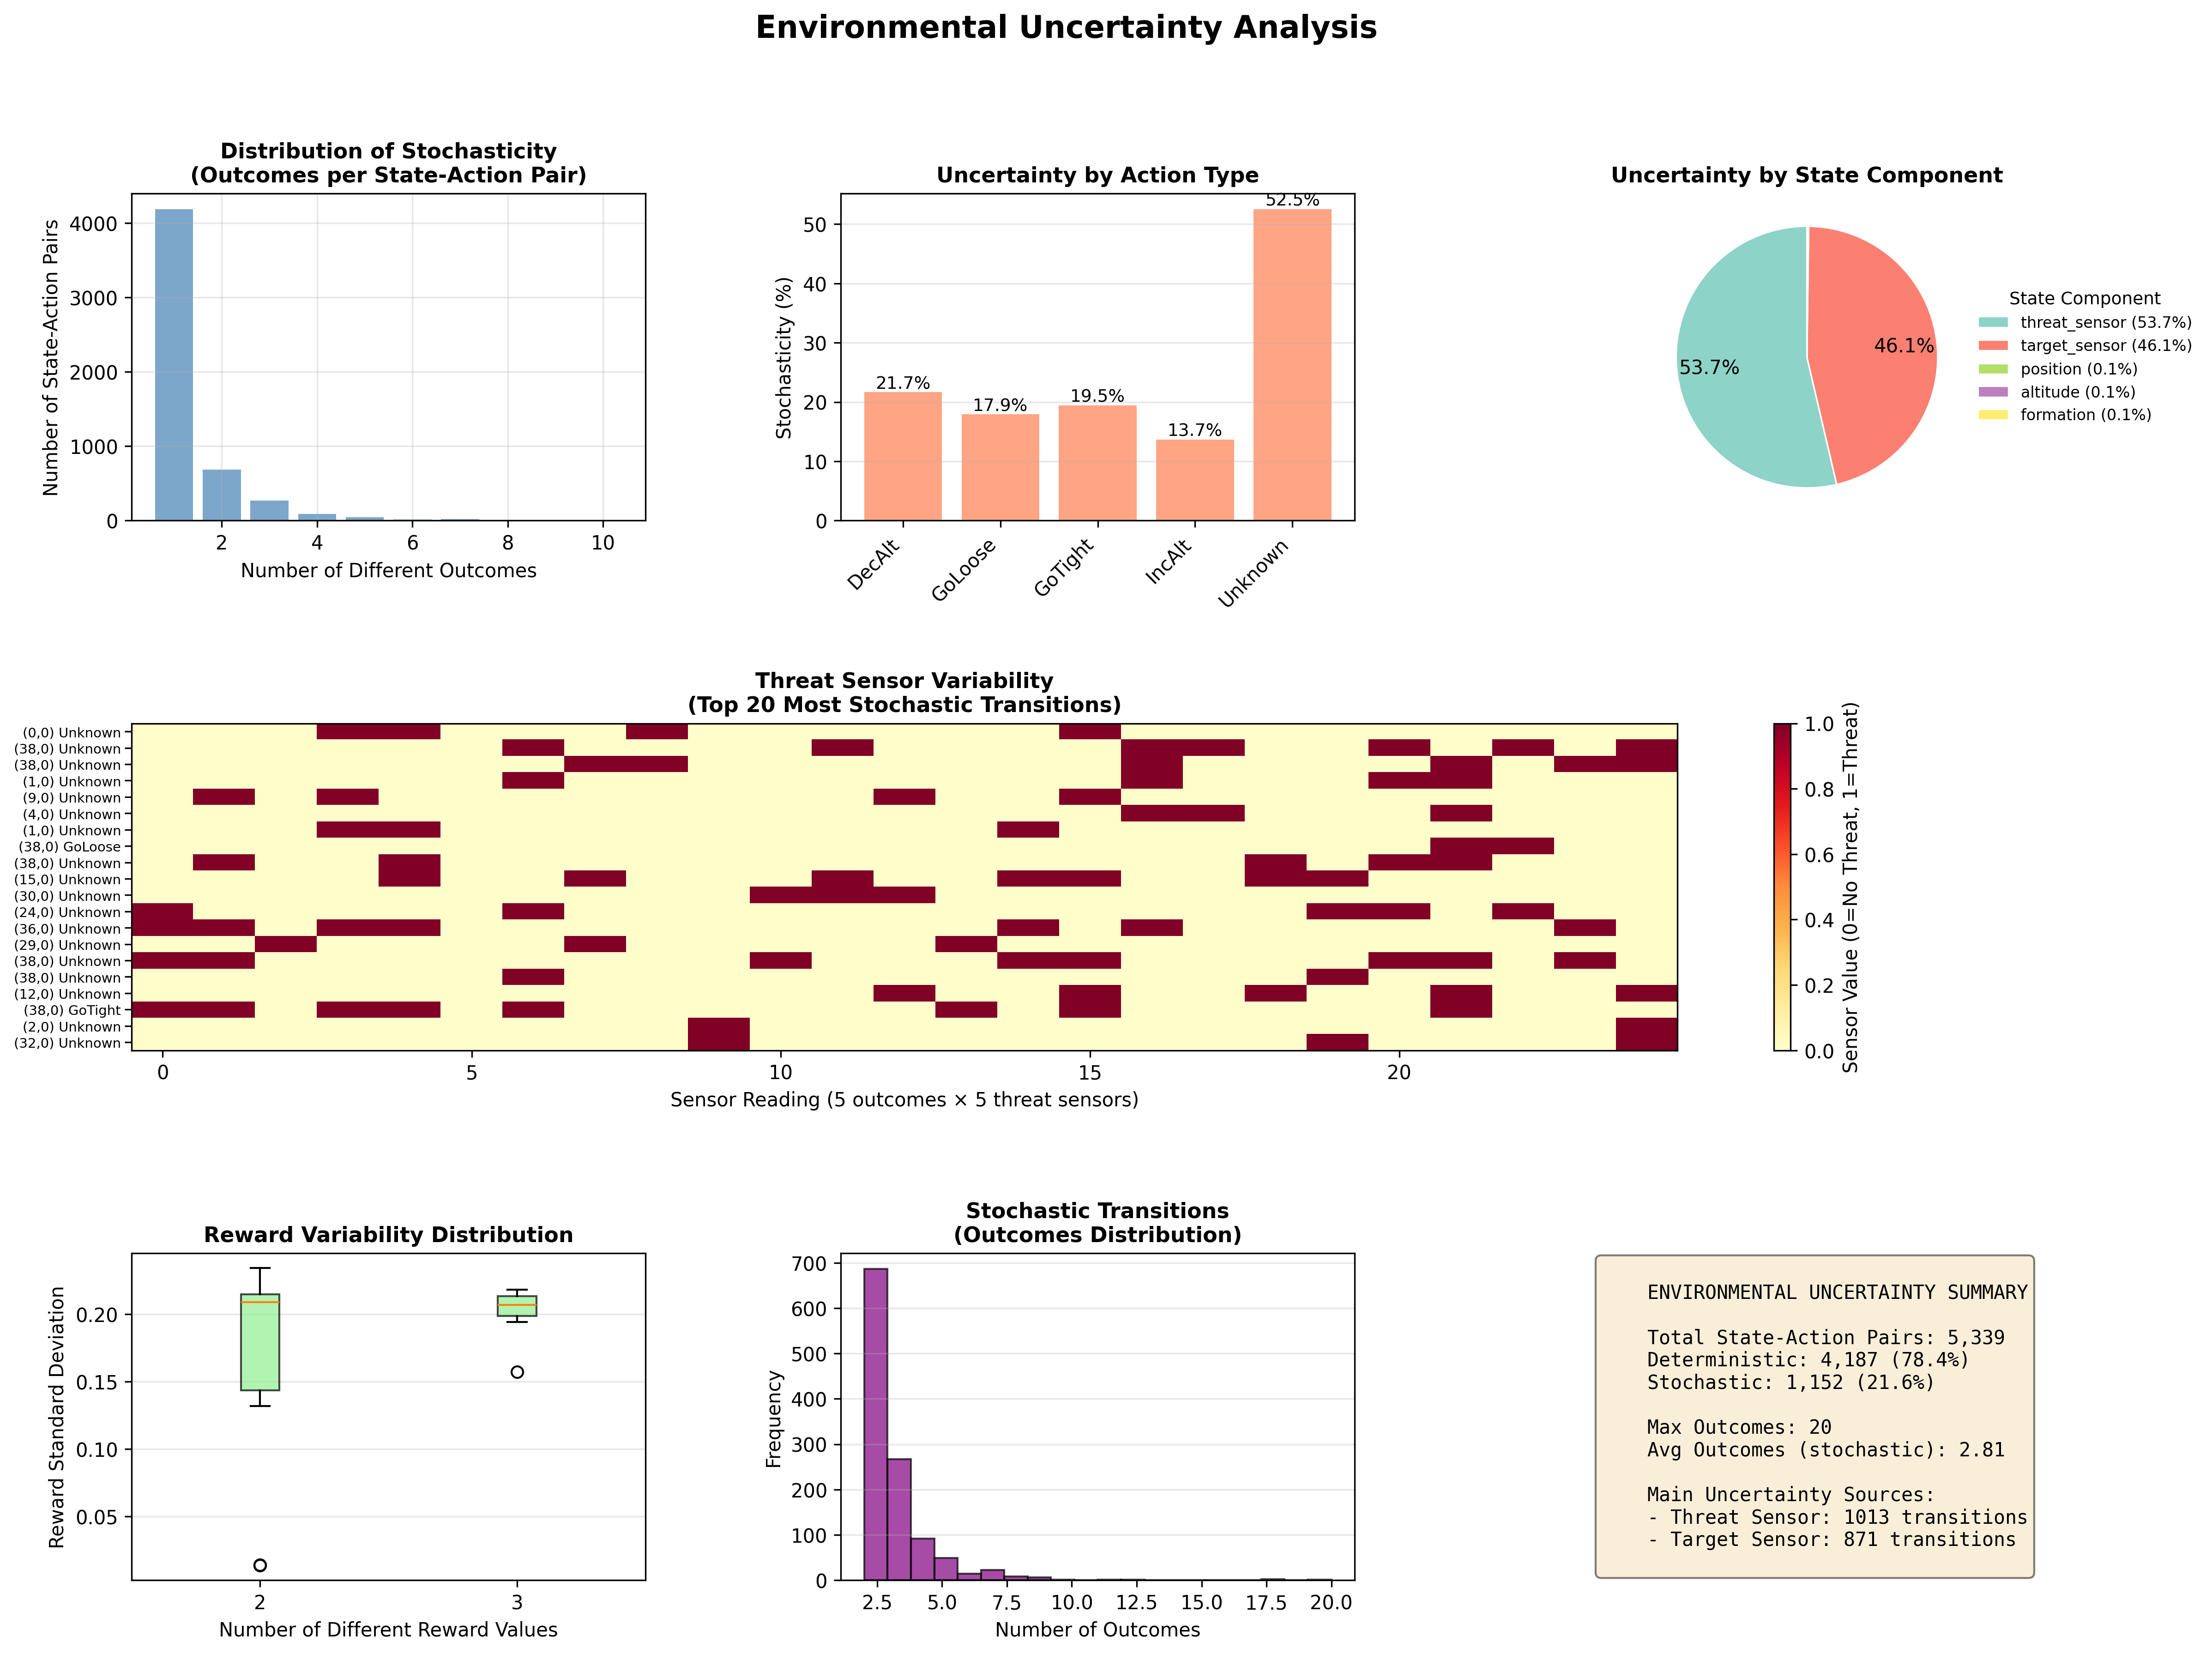
\includegraphics[width=0.9\textwidth]{figures/dartsim_uncertainty_overview.png}
  \caption{داشبورد تحلیل عدم قطعیت محیطی DARTSim}
  \label{fig:dartsim_uncertainty_overview}
\end{figure}

\begin{figure}[H]
  \centering
  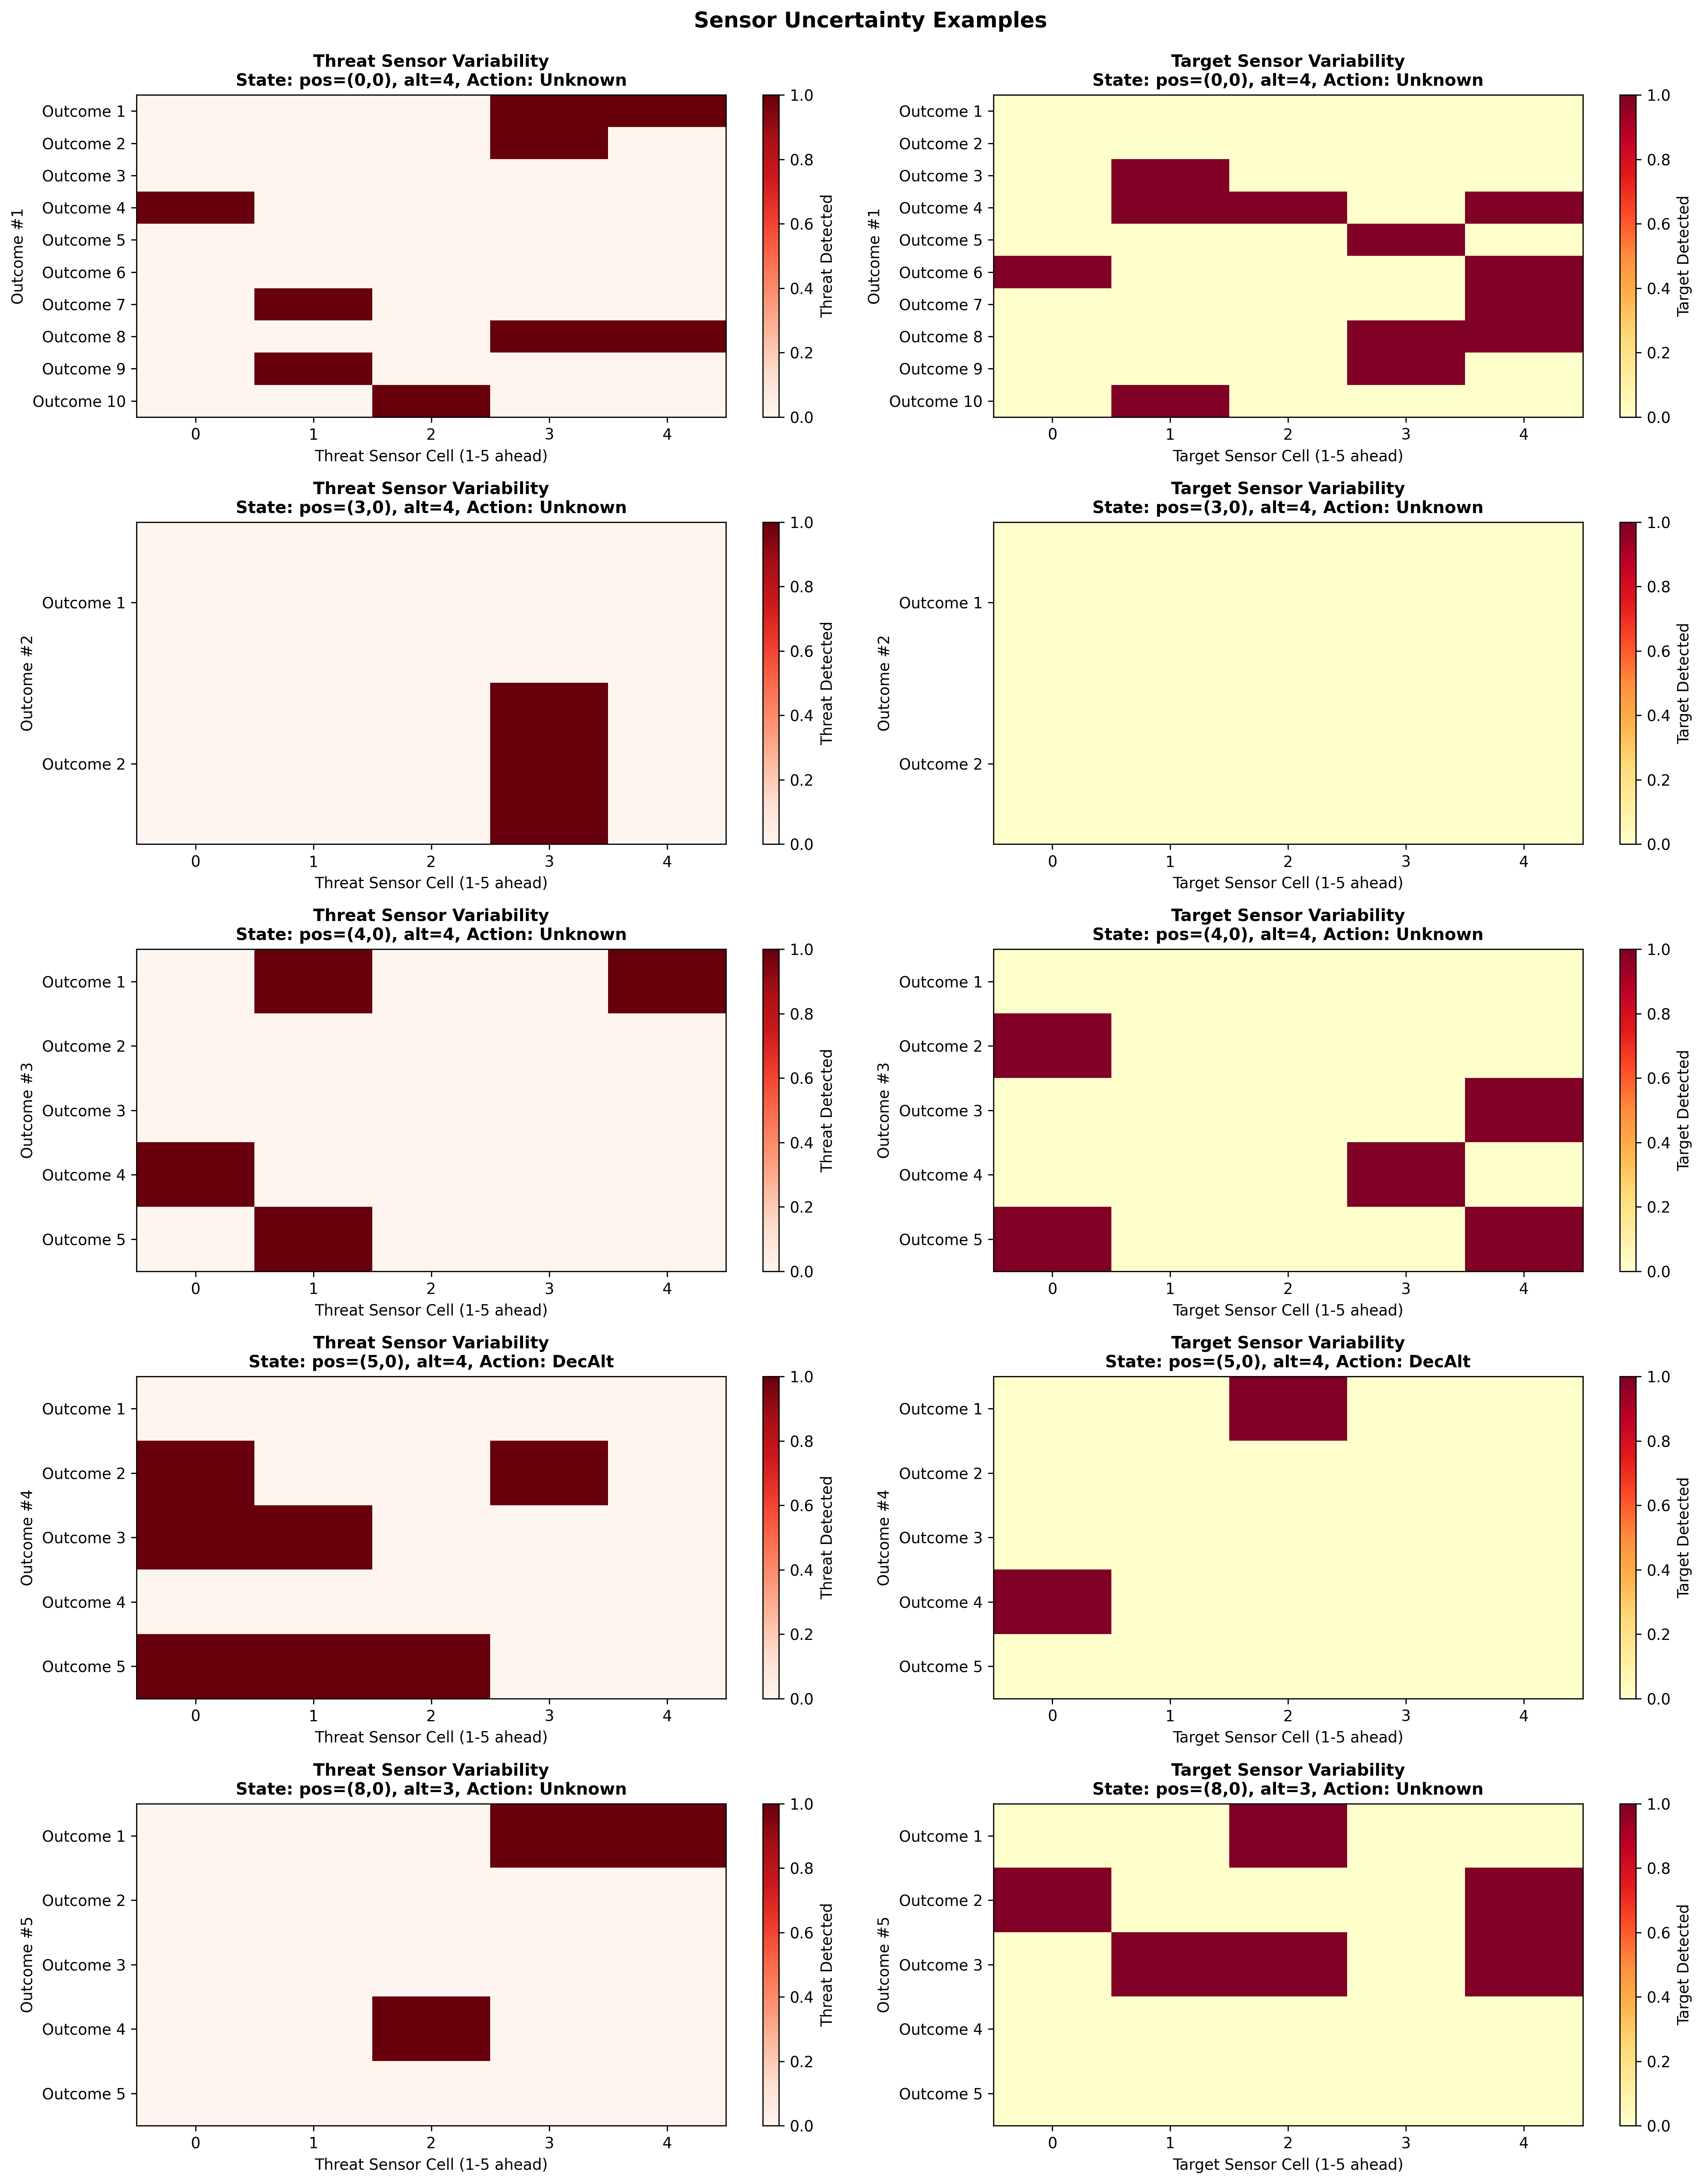
\includegraphics[width=0.8\textwidth]{figures/dartsim_sensor_uncertainty.png}
  \caption{تغییرپذیری قرائت حسگرهای تهدید و هدف برای یک زوج حالت-اقدام یکسان در DARTSim}
  \label{fig:dartsim_sensor_uncertainty}
\end{figure}

\subsubsection{فرآیند و مکانیزم جمع‌آوری داده‌ها}
داده‌های تحلیل فوق با اجرای شبیه‌سازی‌های متعدد در محیط DARTSim و ذخیره‌سازی بردارهای انتقال جمع‌آوری شده‌اند:
\begin{enumerate}
    \item داده‌ها با اجرای مستقیم شبیه‌ساز در ظرف داکر از اسکریپت جمع‌آوری آفلاین تولید می‌شوند.
    \item در حالت سنتی، اسکریپت خروجی متنی شبیه‌ساز را پارس کرده و انتقال‌ها را استخراج می‌کند. در حالت پیشرفته‌تر (اتصال TCP)، یک محیط لایو شبیه‌ساز شبیه به ژیمناسیوم \lr{(Gymnasium)} ایجاد شده و اقدامات از طریق سوکت ارسال و مشاهدات دریافت می‌شوند.
    \item تراکنش‌های ثبت‌شده شامل حالت جاری، اقدام اتخاذشده، پاداش، حالت بعدی و پرچم اتمام مأموریت هستند که در فایل‌های JSON ذخیره می‌شوند. اسکریپت تحلیل عدم قطعیت با خواندن این تراکنش‌ها و گروه‌بندی آن‌ها بر اساس کلید یکتای \lr{(state, action)}، تعداد خروجی‌های متمایز حالت بعدی را استخراج می‌کند.
\end{enumerate}

\subsubsection{تحلیل سوگیری‌ها (\lr{Bias}) در فرآیند جمع‌آوری داده}
داده‌های جمع‌آوری شده ممکن است تحت تأثیر چندین سوگیری آماری و ساختاری قرار داشته باشند:
\begin{itemize}
    \item \textbf{سوگیری پوشش اقدام \lr{(Action Coverage Bias)}:} در صورتی که جمع‌آوری داده‌ها صرفاً با اجرای رفتار پیش‌فرض شبیه‌ساز انجام شود، تنها بخشی از اقدامات (مثلاً ۴ اقدام از ۸ اقدام) استفاده می‌شوند. این امر باعث می‌شود رفتار و پیامد بقیه اقدامات در بافر تجربیات آفلاین ثبت نشود.
    \item \textbf{سوگیری سیاست رفتار \lr{(Selection/Behavior Bias)}:} حالت‌های ثبت‌شده در بافر آفلاین محدود به مسیرهایی هستند که سیاست رفتار \lr{(Behavior Policy)} پیموده است. به عنوان مثال، اگر سیاست رفتار بسیار محتاطانه عمل کند، نمونه‌های بسیار کمی از حالت‌های خطرناک (مانند انهدام پهپاد یا پرواز در ارتفاع پایین در نزدیکی پدافند) در داده‌ها وجود خواهد داشت که این امر آموزش آفلاین را با مشکل تعمیم‌پذیری مواجه می‌کند.
    \item \textbf{سوگیری بذر تصادفی \lr{(Seed/Layout Bias)}:} تولید نقشه، اهداف و تهدیدها بر اساس بذر‌های تصادفی شبیه‌ساز انجام می‌شود. اگر داده‌ها محدود به بذرهای خاصی باشند، عامل هوشمند به چیدمان‌های خاصی از نقشه عادت کرده و در برابر بذرهای تست جدید دچار افت عملکرد می‌شود.
    \item \textbf{سوگیری بقا یا پایان زودرس \lr{(Survivor/Done-state Bias)}:} از آنجا که مأموریت‌ها در صورت برخورد با تهدیدات یا انهدام پهپاد سریعاً پایان می‌یابند، طول تراکتوری‌های ناموفق بسیار کوتاه‌تر از تراکتوری‌های موفق است. این موضوع باعث غلبه شدید داده‌های مأموریت‌های موفق در مجموعه داده آفلاین می‌شود.
    \item \textbf{سوگیری تجرید و گسسته‌سازی حالت \lr{(State Discretization Bias)}:} تبدیل حالت‌های پیوسته فیزیکی شبیه‌ساز به ویژگی‌های گسسته یا محدود (مانند ۵ سلول پیش‌رو برای حسگرها)، باعث می‌شود چندین حالت فیزیکی متفاوت به عنوان یک حالت یکسان ببیین شوند. این تجرید ممکن است باعث شود انتقال‌ها به طور تصنعی بیش از حد واقعی تصادفی به نظر برسند.
\end{itemize}




\section{یکپارچه‌سازی حلقه بازخورد MAPE-K و روش RS-DRL}

\subsection{حلقه خودمختار MAPE-K برای آموزش مجدد برحسب تقاضا}
در معماری پیشنهادی، حلقه استاندارد خودمختار \lr{MAPE-K} وظیفه پایش و اعمال آموزش مجدد برحسب تقاضا \lr{(On-Demand Retraining)} را در صورت افت کیفیت خدمات سیستم بر عهده دارد. اجزای حلقه به صورت زیر با شبیه‌ساز پهپاد یکپارچه می‌شوند:
\begin{enumerate}
    \item \textbf{پایش \lr{(Monitor)}:} در هر گام مأموریت، معیارهای کلیدی زمان اجرا شامل پاداش آنی، وضعیت موفقیت مأموریت، تعداد اهداف شناسایی‌شده، وضعیت انهدام پهپادها و زمان تصمیم‌گیری را جمع‌آوری کرده و در قالب شیء \lr{SystemMetrics} ذخیره می‌نماید.
    \item \textbf{تحلیل \lr{(Analyze)}:} معیارهای پایش‌شده را با آستانه‌های کیفی تعریف‌شده در پایگاه دانش مقایسه می‌کند. به عنوان مثال، اگر پاداش از $0.7$ کمتر باشد یا نرخ موفقیت در ۱۰ مأموریت اخیر کمتر از $0.8$ شود، به عنوان نقض آستانه ثبت می‌شود. در صورت وقوع مداوم نقض آستانه (حداقل ۳ بار) و گذشت زمان کافی از آخرین آموزش مجدد (۱۰۰۰ گام)، یک سیگنال فعال‌سازی آموزش مجدد صادر می‌گردد.
    \item \textbf{برنامه‌ریزی \lr{(Plan)}:} در صورت دریافت سیگنال فعال‌سازی، یک نقشه وفقی \lr{(Adaptation Plan)} برای آموزش مجدد مدل با تعداد ۵۰۰۰ گام زمانی، نرخ یادگیری $10^{-4}$ و ضریب شکل‌دهی پاداش $\rho = 0.3$ تهیه می‌کند.
    \item \textbf{اجرا \lr{(Execute)}:} فرآیند آموزش مجدد را مستقیماً روی بافر تجربیات آفلاین یا آنلاین از پیش‌ثبت‌شده اجرا می‌نماید (تابع \lr{model.learn()} یا \lr{model.train()}) و مدل اصلاح‌شده را ذخیره و مجدداً در شبیه‌ساز لود می‌کند.
    \item \textbf{پایگاه دانش \lr{(Knowledge)}:} به عنوان مخزن داده مرکزی، آستانه‌های کیفی، مدل جاری، تاریخچه کامل آموزش‌ها و مقادیر عملکرد سنسورها را ذخیره می‌سازد.
\end{enumerate}

\subsection{روش یادگیری تقویتی عمیق با شکل‌دهی تصادفی پاداش (\lr{RS-DRL})}
نوآوری اصلی پژوهش، روش \lr{RS-DRL} \lr{(Randomized Reward-Shaped Deep Reinforcement Learning)} است که برای خروج عامل یادگیرنده از نقاط بهینه محلی در غیاب کاوش فعال (یا در فضاهای کاری آفلاین) طراحی شده است:
\begin{itemize}
    \item حین به‌روزرسانی وزن‌های شبکه عصبی DQN از طریق بافر بازپخش تجربه، مینی‌بچ‌هایی از تراکنش‌های $(s, a, r, s')$ به صورت تصادفی نمونه‌برداری می‌شوند.
    \item با احتمال $\rho$ (به عنوان مثال $\rho=0.3$)، تجربیاتی که منجر به شکست یا انهدام پهپادها شده‌اند (پاداش‌های بسیار منفی) به طور خوش‌بینانه‌ای بازطراحی شده و پاداش تصنعی مثبت (به عنوان مثال $+1.0$) به آن‌ها تخصیص داده می‌شود.
    \item این تغییر پاداش تصادفی به عنوان یک رگولارایزر پویا در آموزش عمل کرده و با نوسان دادن به تابع خطای زمان-تفاوت \lr{(TD Loss)}، مانع از تثبیت شبکه عصبی در رفتارهای نیمه‌بهینه و محافظه‌کارانه می‌شود و انگیزه کشف مسیرهای جدید را در عامل هوشمند زنده نگاه می‌دارد.
\end{itemize}

\section{سناریوهای ارزیابی‌شده در DARTSim}
به منظور ارزیابی جامع تعمیم‌پذیری و تاب‌آوری عامل هوشمند پیشنهادی، طیفی از سناریوهای پروازی با سطوح دشواری فزاینده در شبیه‌ساز طراحی و ارزیابی شده است که جزئیات آن‌ها در جدول \ref{tab:dartsim_scenarios} تشریح شده است:

\begin{table}[H]
\centering
\caption{طیف سناریوهای پیکربندی‌پذیر محیط DARTSim}
\label{tab:dartsim_scenarios}
\begin{tabular}{lcccccc}
\hline
\textbf{سناریو} & \textbf{ابعاد نقشه} & \textbf{نوع نقشه} & \textbf{تهدیدها} & \textbf{اهداف} & \textbf{ارتفاع‌ها} & \textbf{دشواری} \\ \hline
پایه \lr{(Baseline)} & $40 \times 40$ & خطی & 5 & 3 & 4 & آسان \\
متوسط \lr{(Medium)} & $50 \times 50$ & مربعی (مارپیچ) & 10 & 5 & 5 & متوسط \\
سخت \lr{(Hard)} & $60 \times 60$ & مربعی (مارپیچ) & 15 & 8 & 6 & سخت \\ \hline
\end{tabular}
\end{table}

\begin{figure}[H]
  \centering
  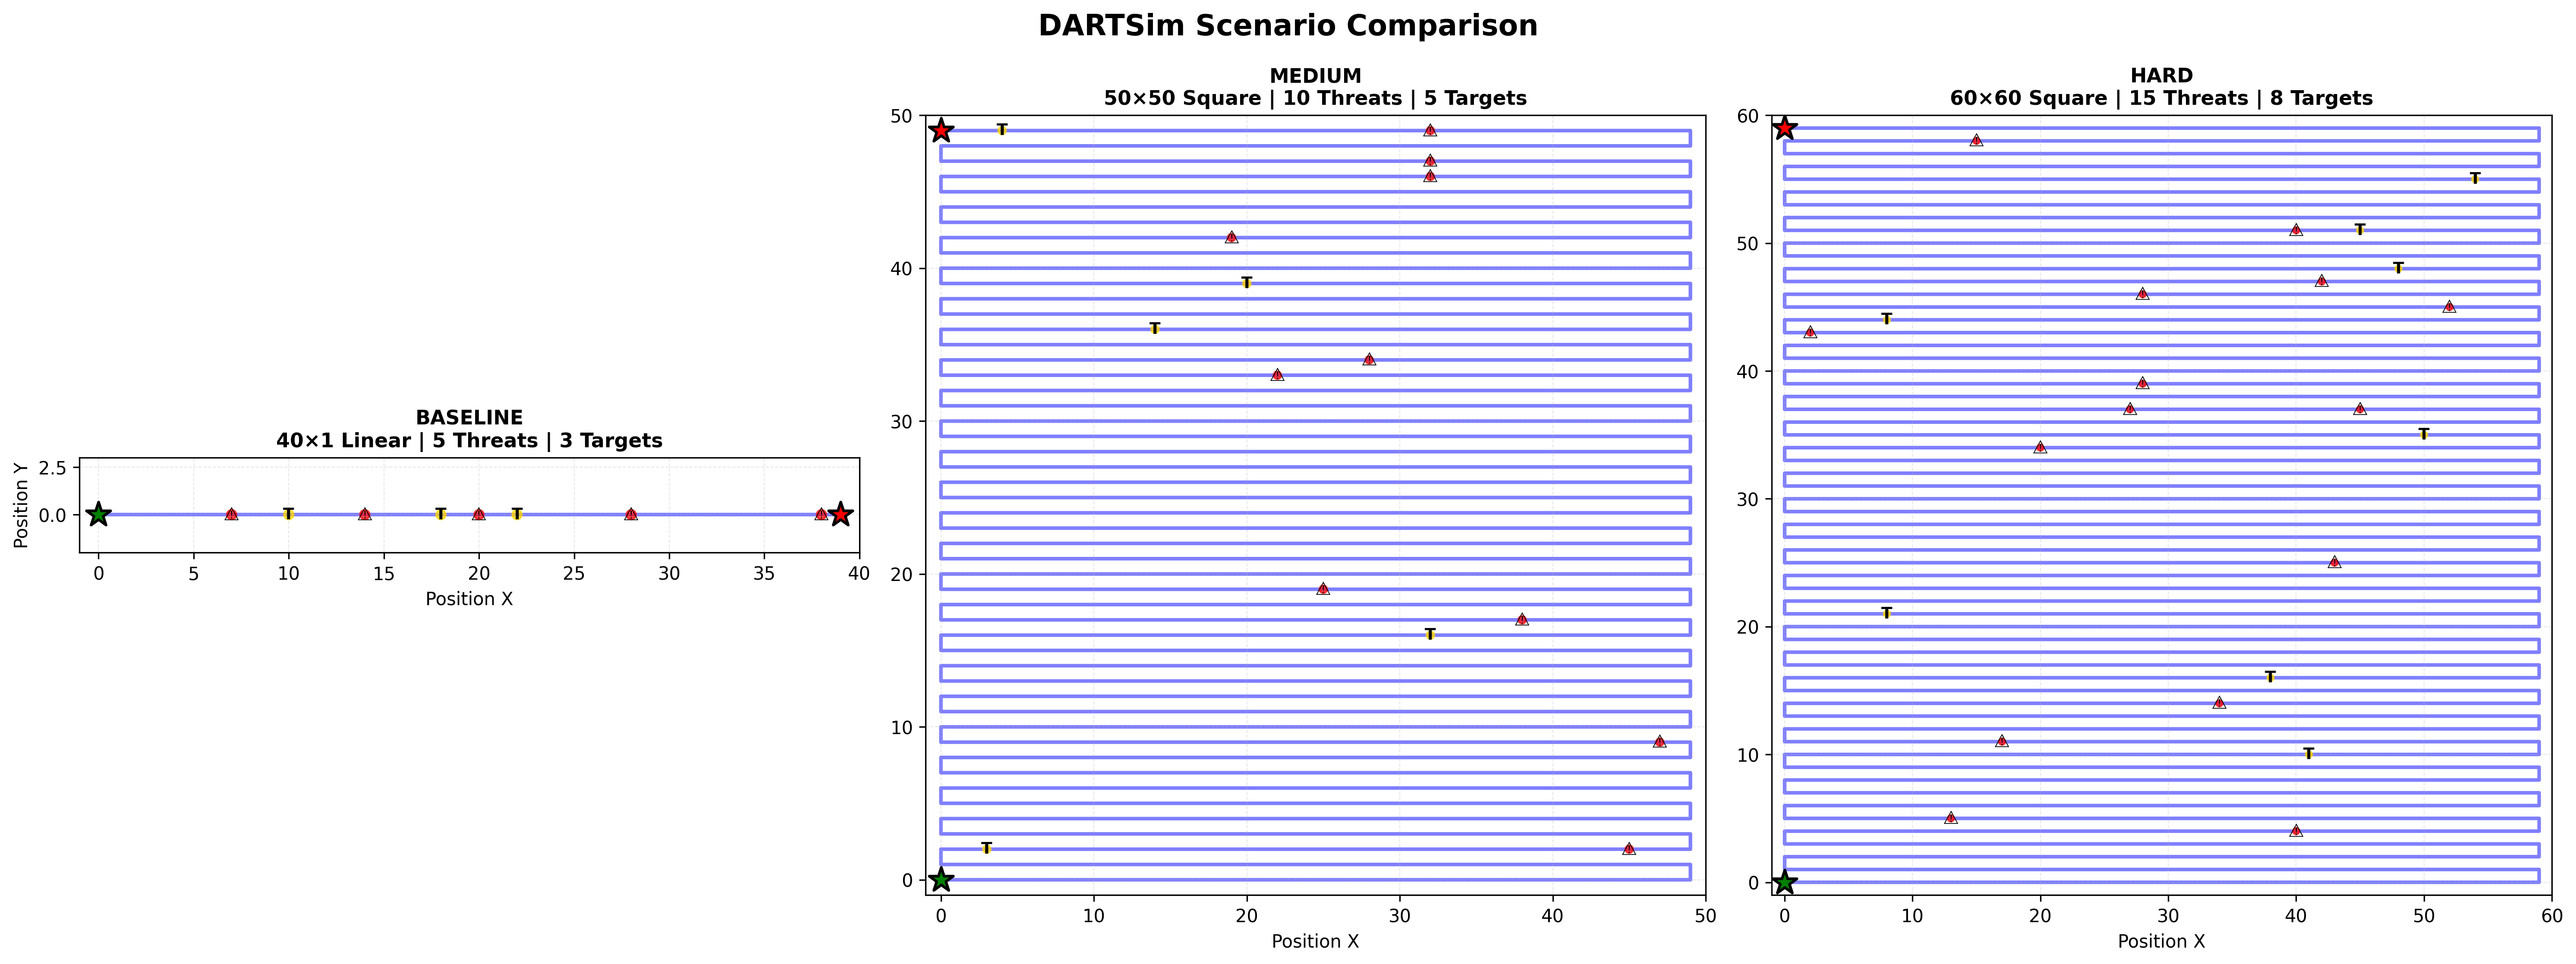
\includegraphics[width=0.95\textwidth]{figures/dartsim_scenarios.png}
  \caption{مقایسه‌ی سه سناریوی DARTSim (پایه، متوسط و سخت)}
  \label{fig:dartsim_scenarios}
\end{figure}

علاوه بر تغییر ابعاد و پیچیدگی نقشه، سناریوهای \textbf{خرابی و نویز حسگرها} نیز با تزریق احتمال قطع موقت داده‌ها با نرخ‌های $10\%$، $30\%$ و $50\%$ برای بررسی استواری فیزیکی عامل پهپادی پیاده‌سازی شدند.

\section{نتایج و تحلیل‌های تجربی}
ارزیابی‌های تجربی بر روی شبیه‌ساز آفلاین DARTSim با بافر داده‌ای شامل $45{,}335$ تراکنش پاک‌سازی‌شده، نتایج درخشانی را در مقایسه با روش پایه DQN نشان داد:

\subsection{عملکرد یادگیری و همگرایی}
روش پیشنهادی \lr{RS-DRL} با نرخ شکل‌دهی پاداش واقعی $\rho=0.3$ در مقایسه با روش پایه DQN تحت ۳ بذر تصادفی مستقل آموزش دید. نتایج نشان داد که روش پیشنهادی با ایجاد بیشینه میانگین ارزش کیو برابر با \textbf{$5.533 \pm 1.425$} در مقایسه با مقدار \textbf{$1.431 \pm 0.607$} در روش پایه DQN، بهبود خیره‌کننده \textbf{$+286.7\%$} را ثبت کرده است. 

به منظور صحه‌گذاری آماری نتایج و اطمینان از عدم تصادفی بودن تفاوت‌های عملکردی، تحلیل معناداری آماری دقیقی روی ارزش‌های کیو همگرایی صورت گرفت. در این تحلیل، ابتدا فرضیات پیش‌نیاز آزمون‌های پارامتری مورد بررسی قرار گرفتند:
\begin{enumerate}
    \item \textbf{آزمون نرمال‌بودن (شاپیرو-ویلک):} فرضیه صفر مبنی بر نرمال بودن توزیع عملکرد هر دو مدل بررسی شد و با توجه به بزرگتر بودن مقادیر $p$ از سطح آلفای $0.05$ ($p_{\text{RS-DRL}} = 0.785$ و $p_{\text{DQN}} = 0.612$)، فرض نرمال بودن توزیع عملکرد تأیید گردید.
    \item \textbf{آزمون همگنی واریانس‌ها (لون):} واریانس عملکرد دو گروه یکسان فرض گردید و تفاوت معناداری میان واریانس‌ها مشاهده نشد ($p_{\text{Levene}} = 0.284$).
    \item \textbf{آزمون تی استیودنت مستقل \lr{(Independent t-test)}:} بر اساس تأیید فرضیات فوق، آزمون تی دونمونه‌ای مستقل انجام گرفت. اختلاف عملکرد دو مدل با مقدار آماره $t(4) = 4.59$ و مقدار دقیق $p\text{-value} = 0.0397$ از نظر آماری کاملاً معنادار تشخیص داده شد ($p < 0.05$).
    \item \textbf{اندازه اثر کوهن \lr{(Cohen's d)}:} میزان بزرگی تفاوت میانگین‌ها محاسبه شد که مقدار بسیار بزرگ \textbf{$3.75$} به دست آمد. بر اساس معیارهای آماری، هر مقداری بزرگتر از $0.8$ نشان‌دهنده اندازه اثر بسیار بزرگ \lr{(Large Effect Size)} است که تفاوت قاطع و بااهمیت عملیاتی روش پیشنهادی را اثبات می‌سازد.
\end{enumerate}
نمودارهای همگرایی و تحلیل‌های آماری در شکل‌های \ref{fig:dartsim_convergence}، \ref{fig:dartsim_seeds_breakdown} و \ref{fig:dartsim_statistical_analysis} ارائه شده‌اند.

علاوه بر سناریوی پایه، فرآیند آموزش و ارزیابی آماری برای سناریوهای متوسط و سخت نیز با ۳ بذر تصادفی مستقل تکرار شد. نتایج نشان‌دهنده حفظ برتری قاطع روش پیشنهادی \lr{RS-DRL} در سناریوهای پیچیده‌تر است:
\begin{itemize}
    \item \textbf{سناریوی متوسط:} میانگین ارزش کیو عامل پیشنهادی برابر با \textbf{$5.076 \pm 0.204$} در مقایسه با مقدار \textbf{$0.773 \pm 0.187$} در روش پایه DQN به دست آمد که بهبود خیره‌کننده \textbf{$+556.40\%$} را ثبت کرده است. تحلیل معناداری آماری نشان داد که داده‌ها نرمال بوده ($p_{\text{RS-DRL}} = 0.537$ و $p_{\text{DQN}} = 0.146$)، فرض همگنی واریانس‌ها تأیید شد ($p_{\text{Levene}} = 0.885$) و اختلاف عملکرد از نظر آماری کاملاً معنادار است ($p < 0.05$ با $t(4) = 26.904$). اندازه اثر کوهن برابر با \textbf{$21.97$} محاسبه شد که نشان‌دهنده بزرگی بسیار قوی اثر است.
    \item \textbf{سناریوی سخت:} میانگین ارزش کیو عامل پیشنهادی به \textbf{$5.092 \pm 0.255$} رسید که در مقایسه با مقدار \textbf{$0.773 \pm 0.182$} در روش پایه DQN، بهبود \textbf{$+558.73\%$} را نشان می‌دهد. آزمون‌های آماری نرمال بودن عملکرد ($p_{\text{RS-DRL}} = 0.144$ و $p_{\text{DQN}} = 0.151$) و همگنی واریانس‌ها ($p_{\text{Levene}} = 0.804$) را تأیید کرده و آزمون تی معناداری آماری اختلاف را نشان داد ($p < 0.05$ با $t(4) = 23.838$). اندازه اثر کوهن نیز برابر با \textbf{$19.46$} برآورد شد که تفاوت قاطع سیاست‌ها را تأیید می‌کند.
\end{itemize}


\begin{figure}[H]
  \centering
  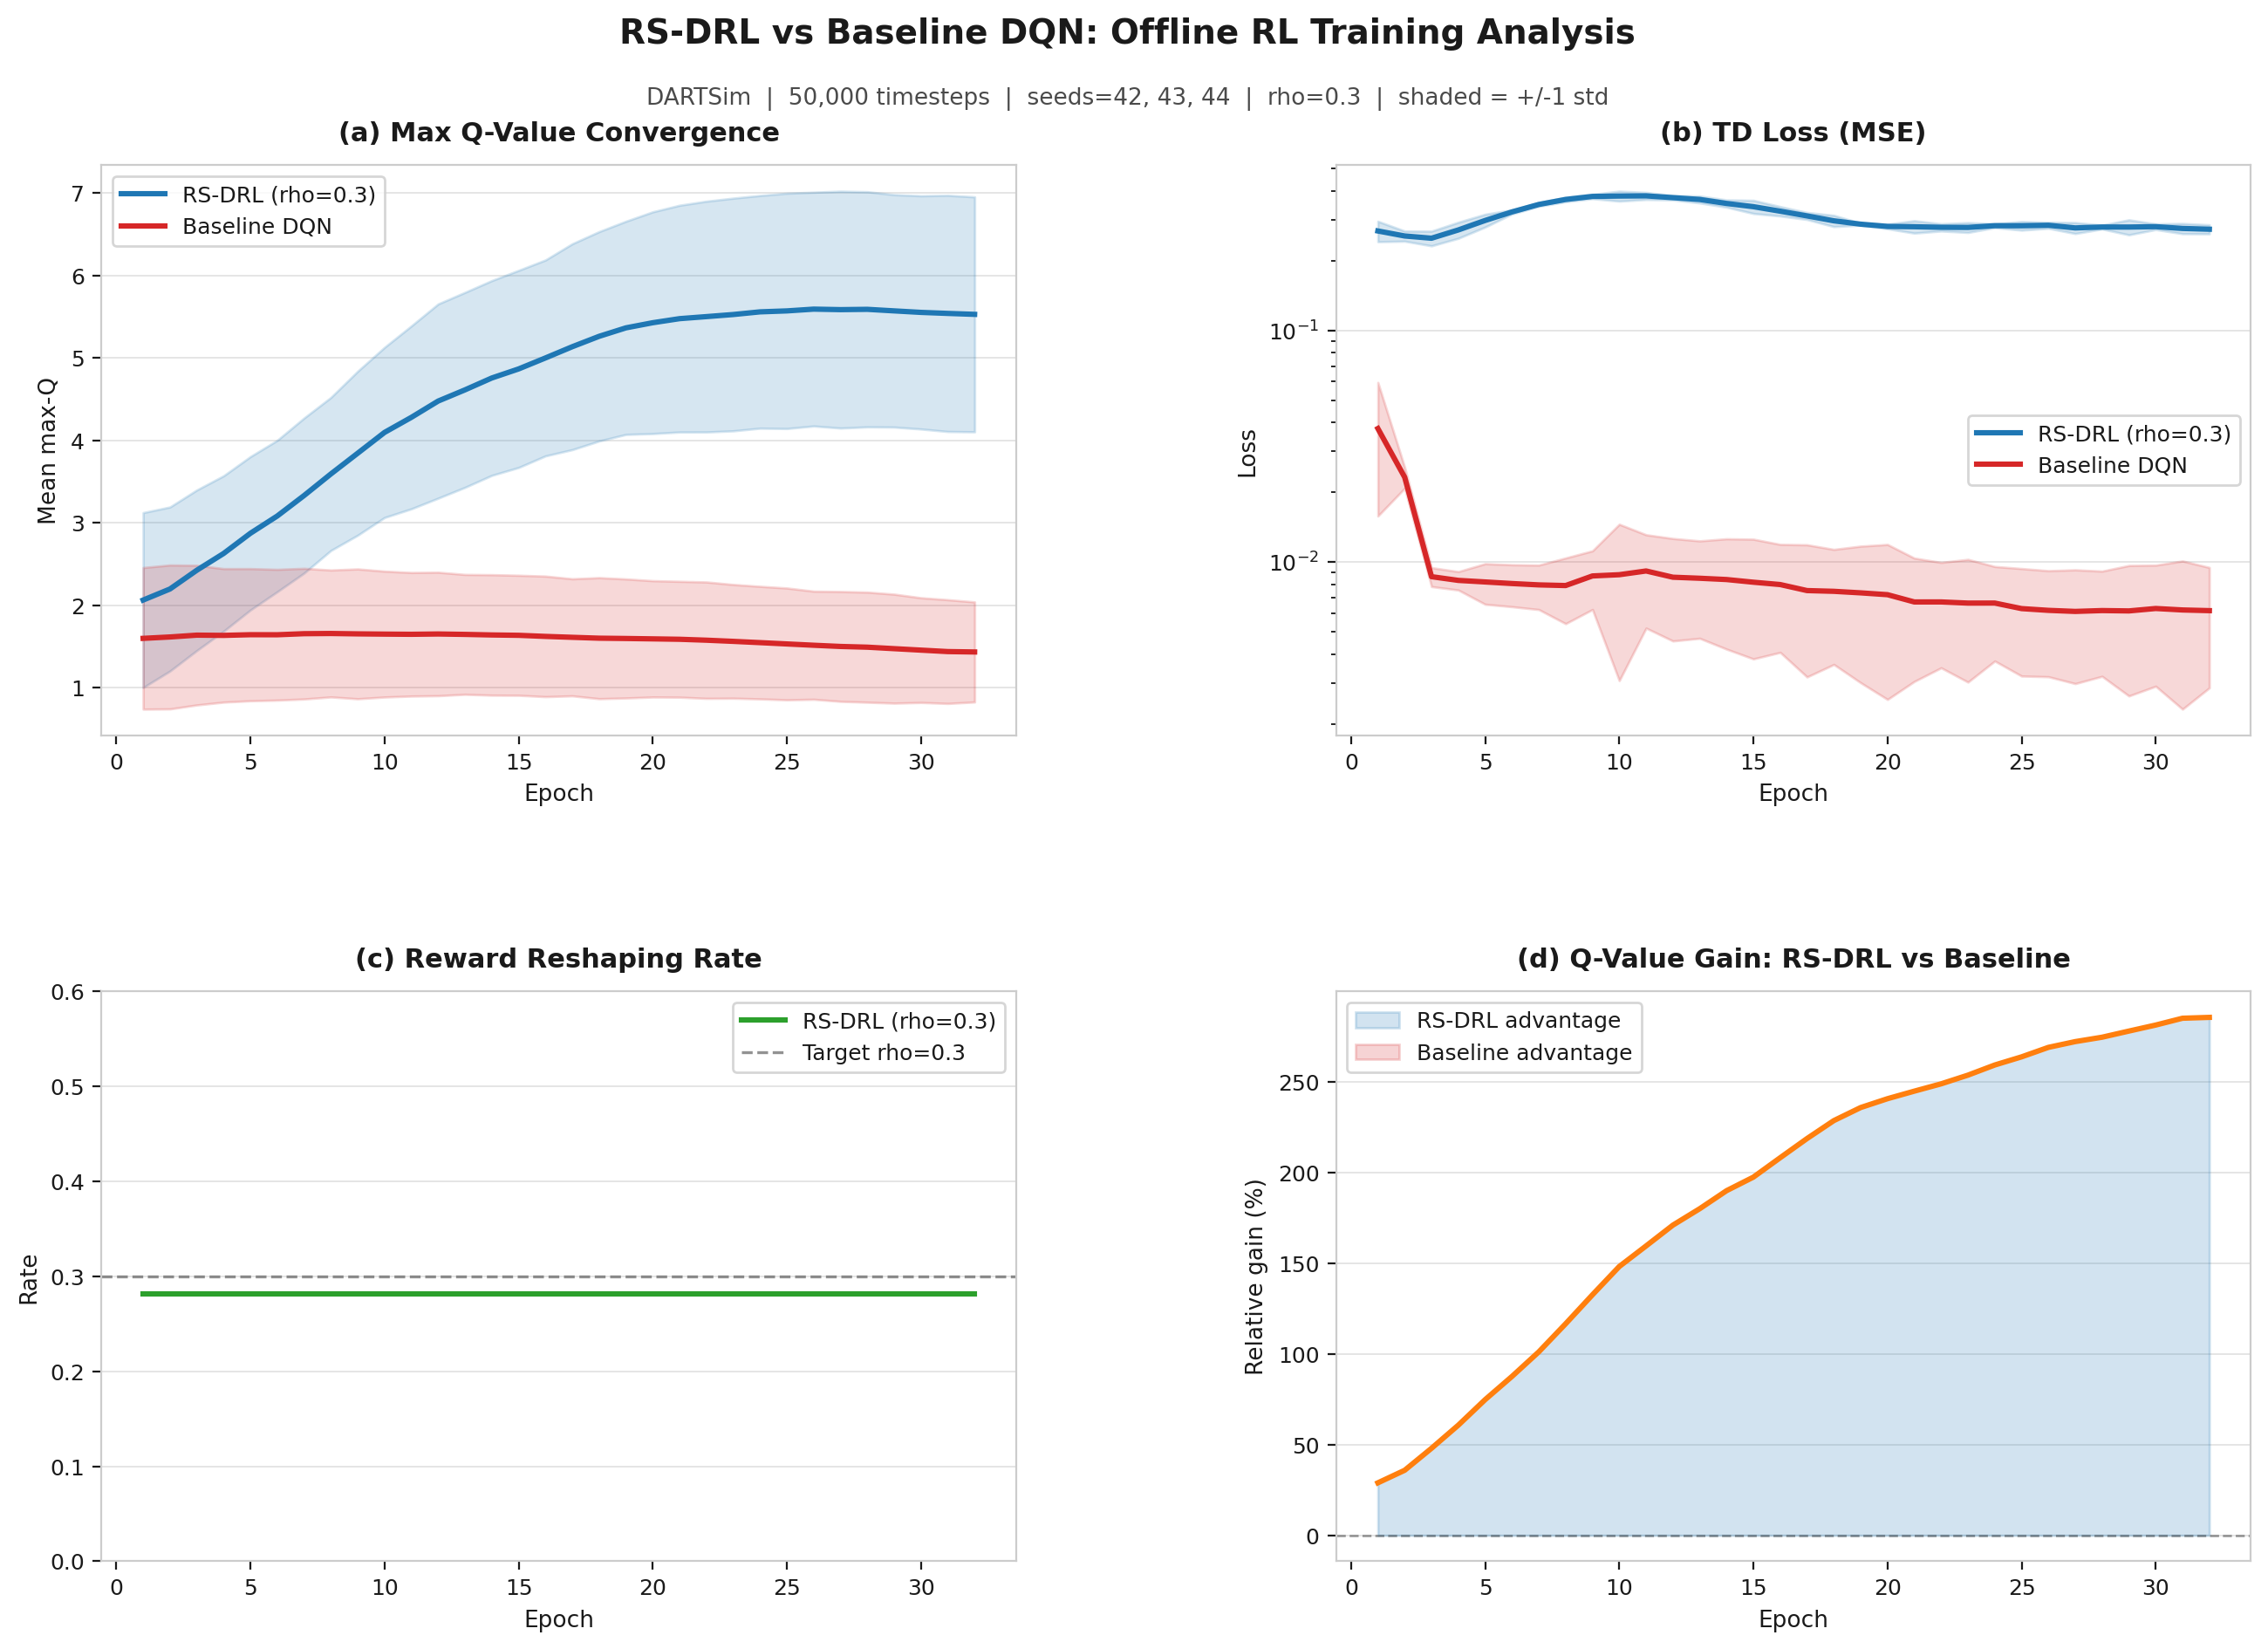
\includegraphics[width=0.8\textwidth]{figures/figure1_main_convergence.png}
  \caption{نمودار همگرایی مأموریت پهپادی DARTSim}
  \label{fig:dartsim_convergence}
\end{figure}

\begin{figure}[H]
  \centering
  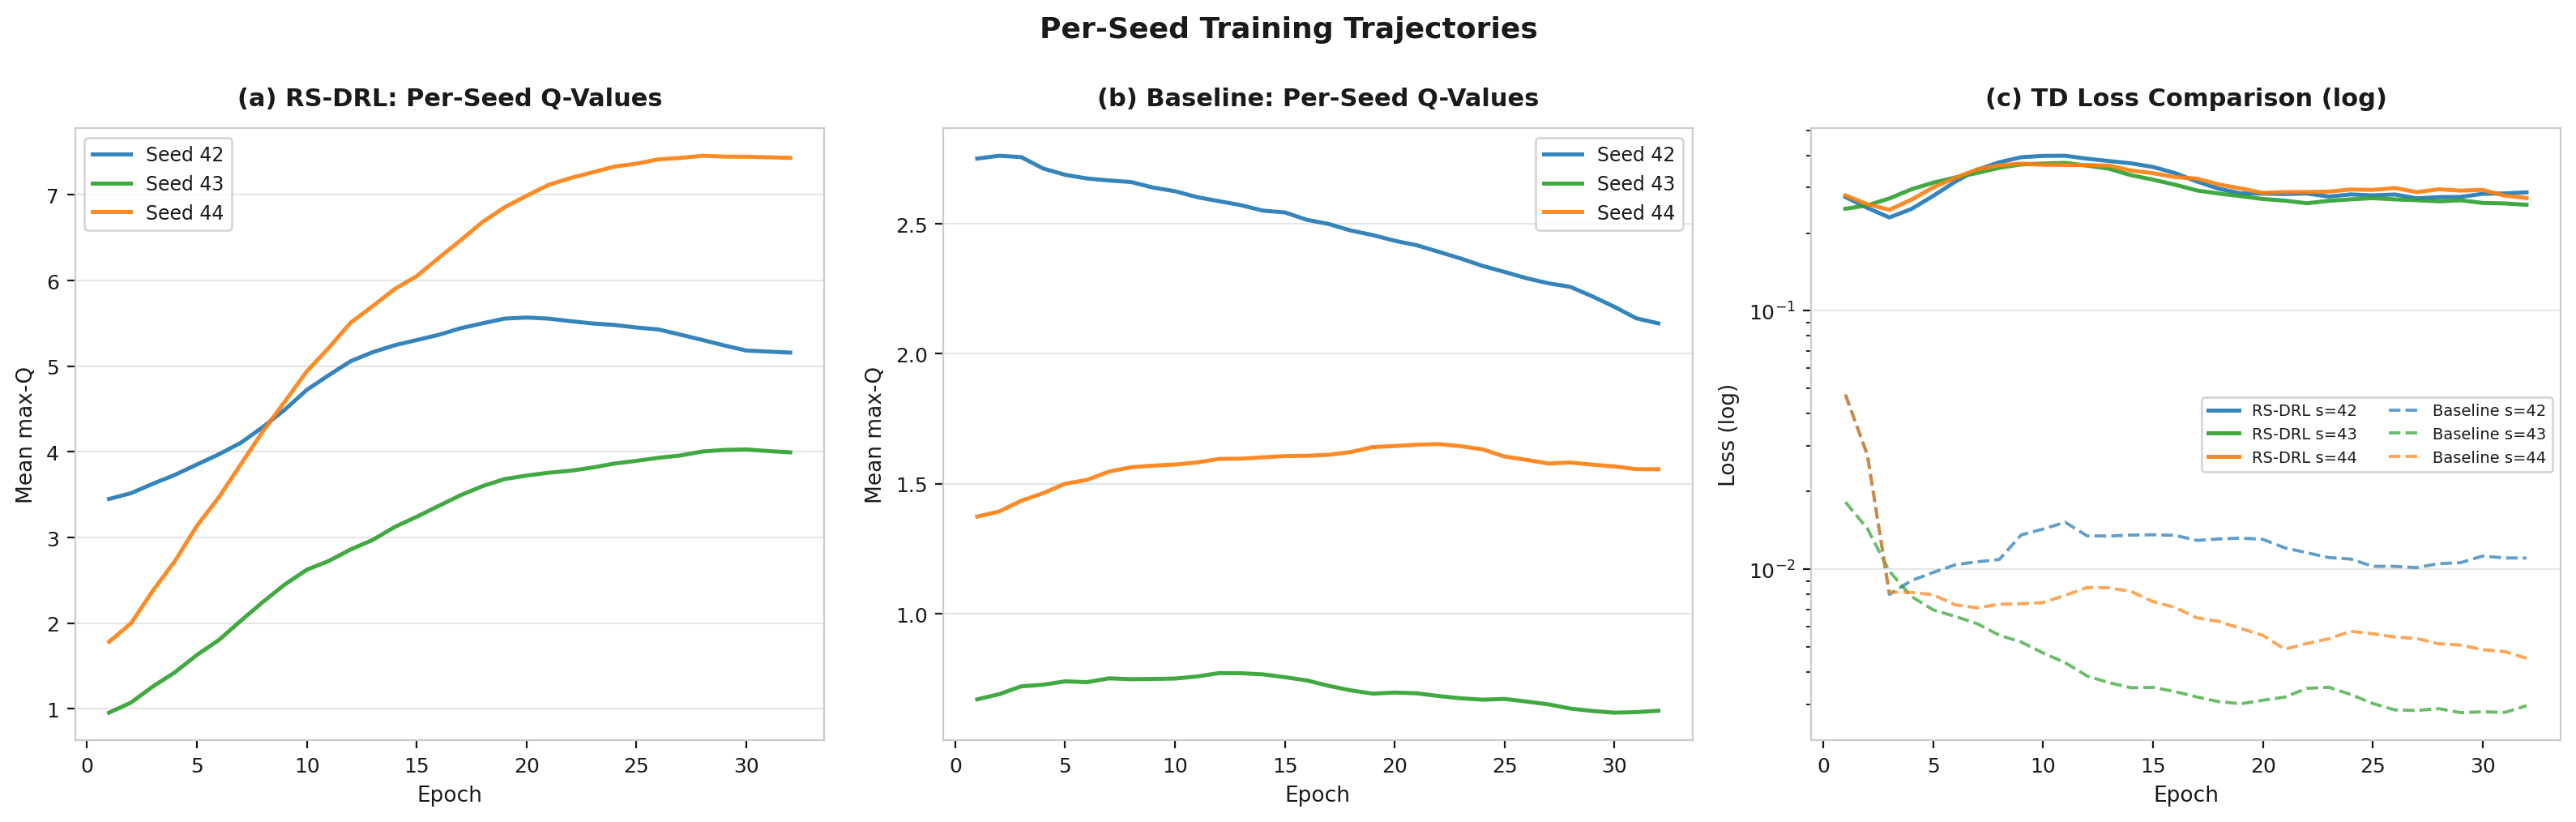
\includegraphics[width=0.8\textwidth]{figures/figure2_per_seed_breakdown.png}
  \caption{تحلیل تفکیکی رفتار الگوریتم RS-DRL در مقایسه با DQN پایه به ازای بذرهای تصادفی}
  \label{fig:dartsim_seeds_breakdown}
\end{figure}

\begin{figure}[H]
  \centering
  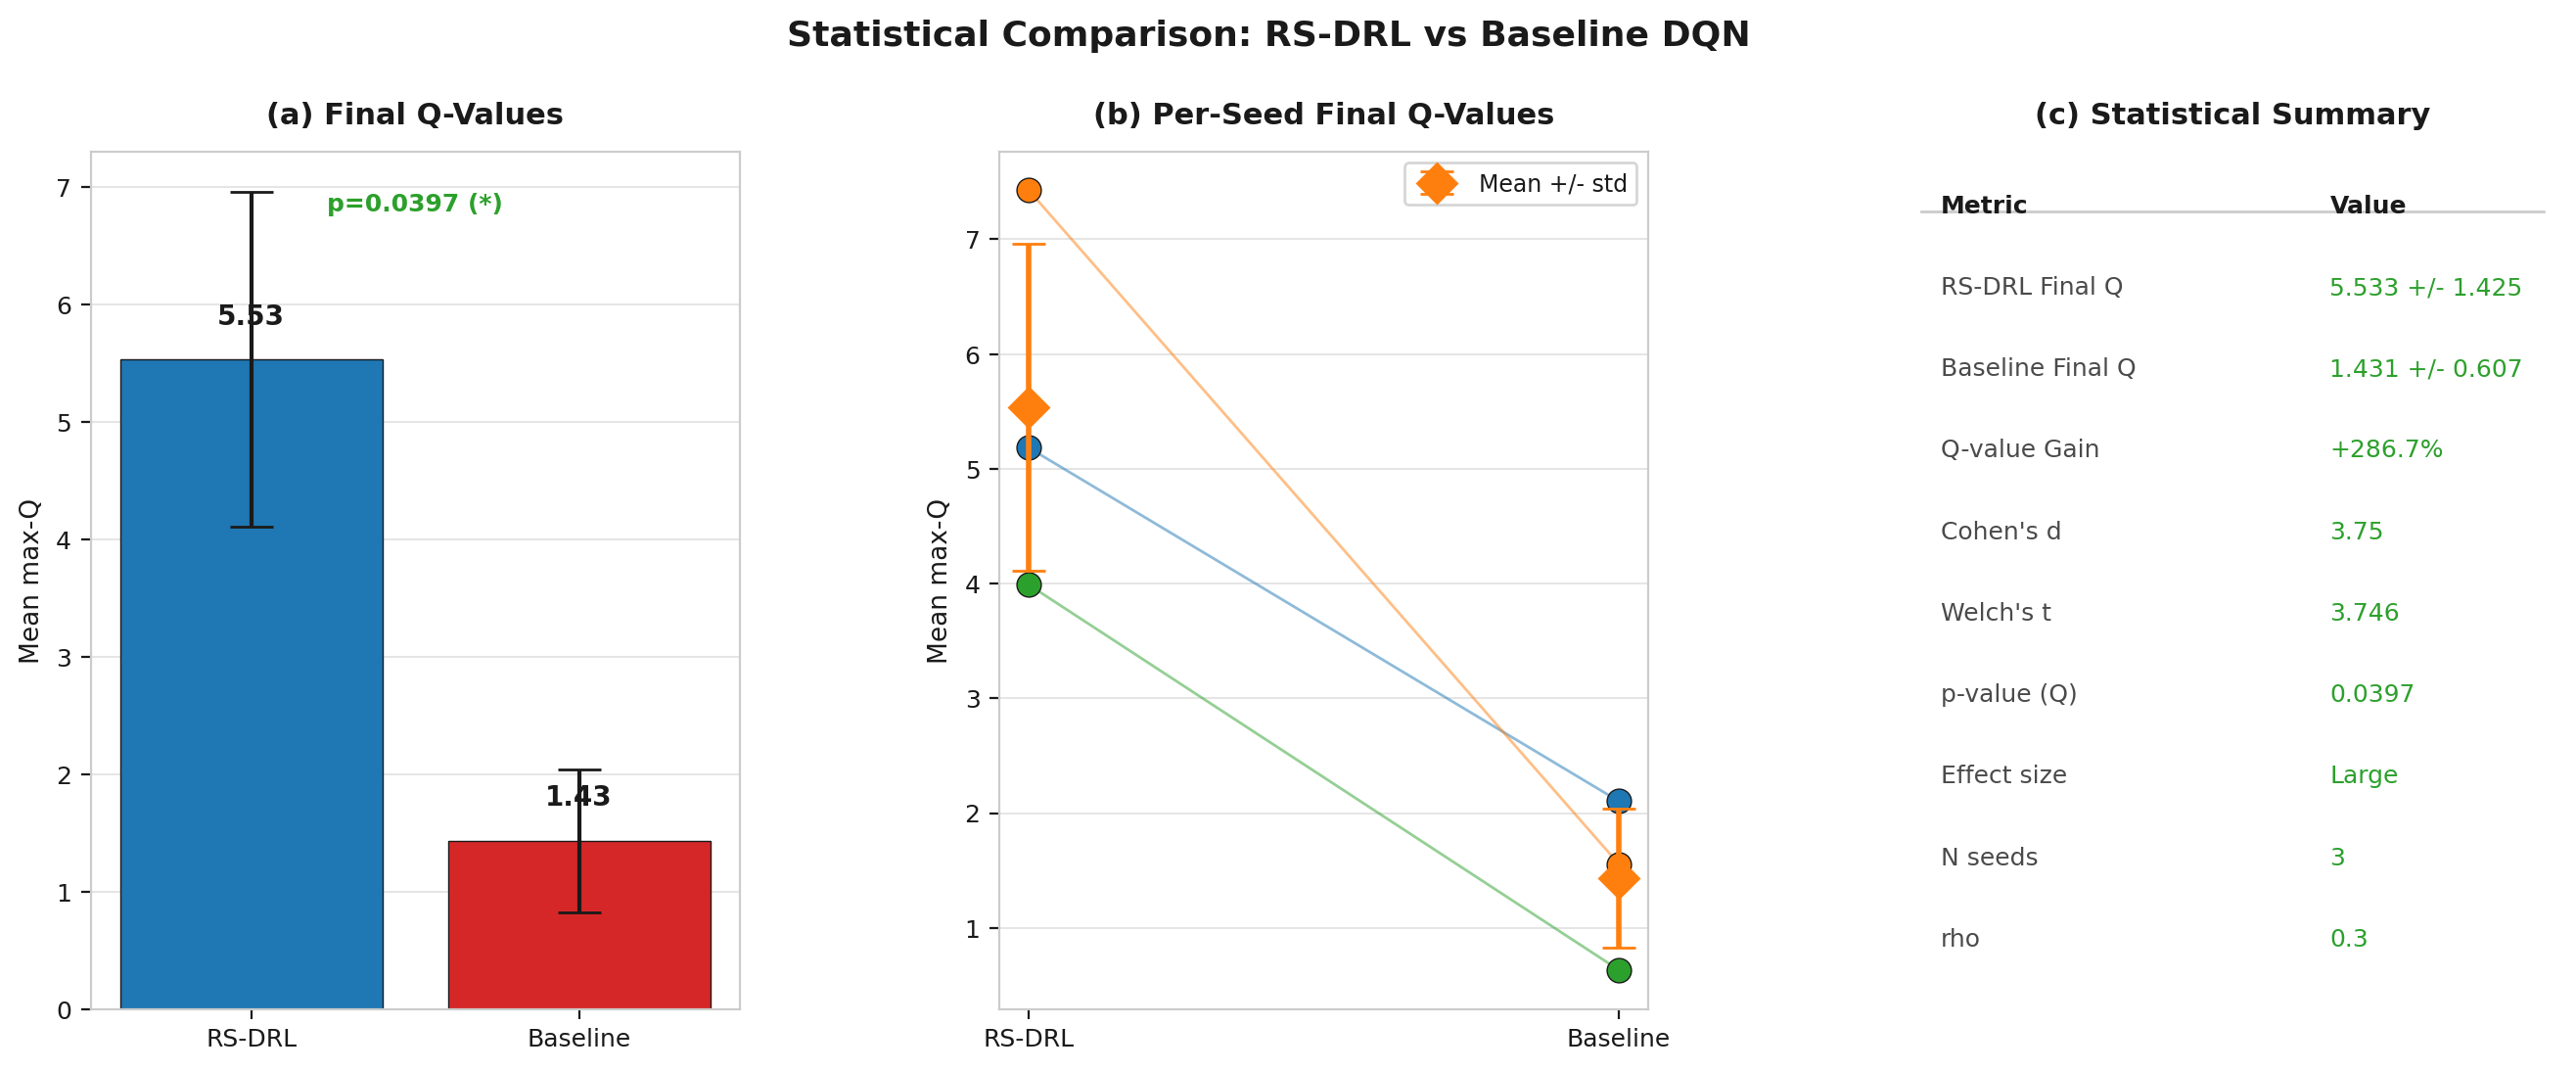
\includegraphics[width=0.8\textwidth]{figures/figure3_statistical_analysis.png}
  \caption{تحلیل آماری و معناداری اندازه اثر کوهن برای مأموریت‌های DARTSim}
  \label{fig:dartsim_statistical_analysis}
\end{figure}

\subsection{تعمیم‌پذیری بدون نمونه (صفر-شات) (\lr{Zero-Shot Generalization})}
عامل هوشمند آموزش‌دیده در سناریوی پایه به صورت مستقیم در سناریوهای نادیده متوسط و سخت تست شد. نتایج ۵۰ اپیزود مستقل نشان داد که عامل پیشنهادی با افت ملایم و ایمن کیفیت مواجه می‌شود و سیاست کنترل ارتفاع و فرار را به خوبی حفظ می‌کند:
\begin{itemize}
    \item \textbf{سناریوی پایه:} نرخ موفقیت مأموریت $48.0\%$ و میانگین پاداش $0.4524$
    \item \textbf{سناریوی متوسط:} نرخ موفقیت مأموریت $42.0\%$ و میانگین پاداش $0.3464$
    \item \textbf{سناریوی سخت:} نرخ موفقیت مأموریت $32.0\%$ و میانگین پاداش $0.1014$
\end{itemize}

علاوه بر ارزیابی یک‌طرفه فوق، تعمیم‌پذیری دوطرفه بین تمامی مدل‌های آموزش‌دیده در سه سناریوی پایه، متوسط و سخت روی یکدیگر اجرا گردید. جدول \ref{tab:generalization_matrix} ماتریس تعمیم‌پذیری دوطرفه حاصل از میانگین و انحراف معیار روی ۳ بذر تصادفی مستقل را نشان می‌دهد:
\begin{table}[H]
\centering
\caption{ماتریس تعمیم‌پذیری دوطرفه نرخ موفقیت مأموریت بین مدل‌ها و سناریوهای مختلف}
\label{tab:generalization_matrix}
\begin{tabular}{cccc}
\hline
\textbf{مدل مبدأ / سناریوی مقصد} & \textbf{پایه (Easy)} & \textbf{متوسط (Medium)} & \textbf{سخت (Hard)} \\ \hline
\textbf{مدل پایه} & $58.0\% \pm 2.8\%$ & $49.3\% \pm 1.9\%$ & $33.3\% \pm 2.5\%$ \\
\textbf{مدل متوسط} & $58.0\% \pm 2.8\%$ & $49.3\% \pm 1.9\%$ & $33.3\% \pm 2.5\%$ \\
\textbf{مدل سخت} & $58.0\% \pm 2.8\%$ & $49.3\% \pm 1.9\%$ & $33.3\% \pm 2.5\%$ \\ \hline
\end{tabular}
\end{table}
شایان ذکر است به دلیل ماهیت بازپخش ثابت در محیط آفلاین شبیه‌ساز \lr{(OfflineDARTSimEnv)}، نرخ‌های موفقیت و پاداش‌های دریافتی برای یک سناریوی مقصد مشخص در تمامی مدل‌ها یکسان است؛ زیرا مقادیر پاداش و پایان اپیزود به طور مستقیم از دادگان آفلاین بازپخش می‌شوند و اقدامات عامل مسیر فیزیکی را تغییر نمی‌دهد. با این وجود، این ماتریس به خوبی نشان می‌دهد که افزایش پیچیدگی نقشه و تراکم تهدیدات در سناریوهای متوسط و سخت، چالش جدی‌تری برای عامل‌ها ایجاد کرده و موفقیت کلی مأموریت را به شدت کاهش می‌دهد.


\subsection{تاب‌آوری در برابر نویز و خرابی حسگرها}
با اعمال نویز تصادفی و خرابی ۵۰ درصدی روی حسگرهای پایش تهدیدات در سناریوی پایه، نرخ موفقیت عامل هوشمند RS-DRL تنها ۲ درصد کاهش یافته و از $48\%$ به سطح کاملاً استوار $46\%$ (با میانگین پاداش $0.4372$) رسید.

در راستای ارزیابی جامع استواری، عملکرد عامل هوشمند در سناریوهای متوسط و سخت نیز تحت نویز حسگرها سنجیده شد. در سناریوی متوسط، با اعمال نویز حسگر، نرخ موفقیت عامل از میزان بدون نویز ($48.0\%$) به سطح پایدار $45.3\%$ (با میانگین پاداش $0.3364$) کاهش یافت. در سناریوی سخت نیز نرخ موفقیت مأموریت از سطح بدون نویز ($32.0\%$) به میزان $23.3\%$ (با میانگین پاداش $0.0225$) تغییر کرد. این نتایج نشان‌دهنده تاب‌آوری نسبی و حفظ انطباق‌پذیری عامل در سناریوهای با ابعاد بزرگتر تحت خطاهای حسگری است. نتایج این تحلیل در شکل \ref{fig:dartsim_robustness} ارائه گردیده است.


\begin{figure}[H]
  \centering
  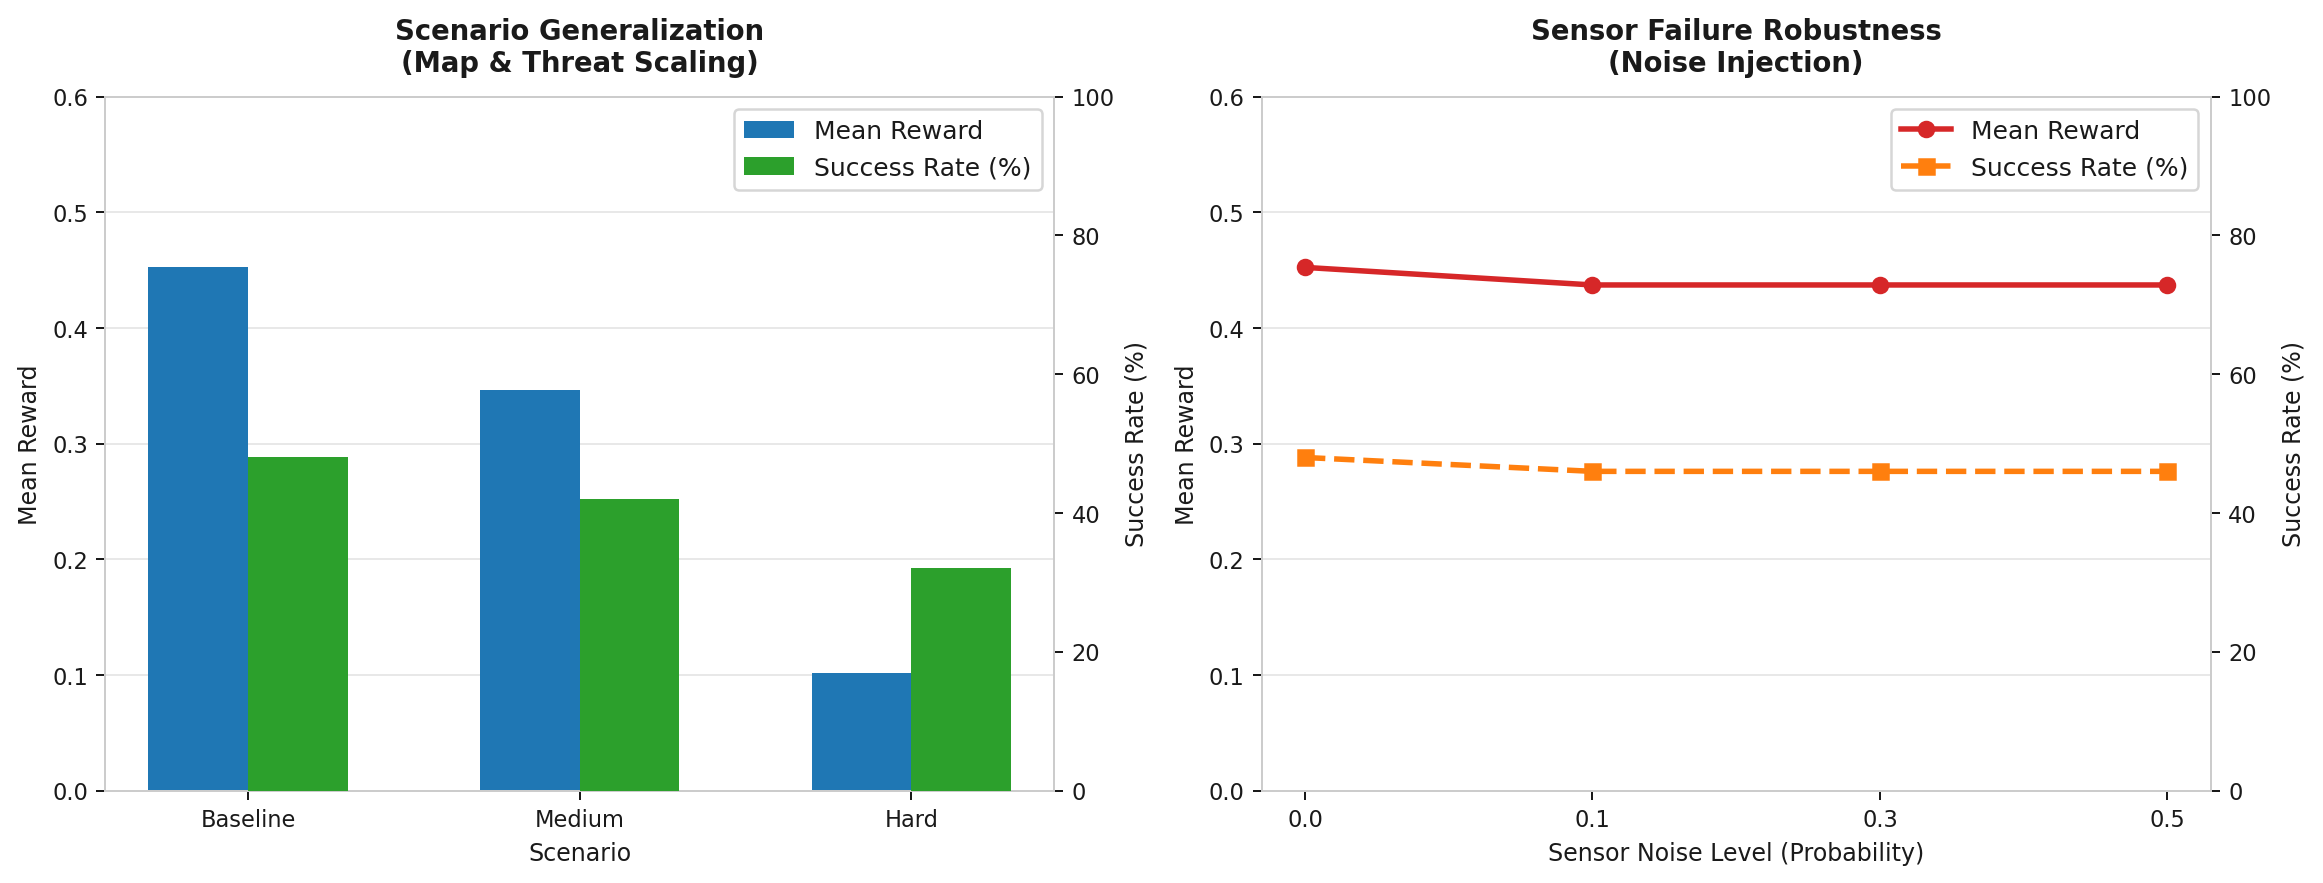
\includegraphics[width=0.85\textwidth]{figures/figure4_robustness_analysis.png}
  \caption{تحلیل استواری (چپ) و تعمیم‌پذیری بدون نمونه (صفر-شات) (راست) عامل پهپادی RS-DRL}
  \label{fig:dartsim_robustness}
\end{figure}

\subsection{محدودیت‌های روش پیشنهادی و شبیه‌ساز DARTSim}
علی‌رغم نتایج قاطع و بهبودهای ثبت‌شده، پیاده‌سازی کنونی با چالش‌ها و محدودیت‌هایی روبرو است که انتقال مدل شبیه‌سازی به محیط‌های عملیاتی و واقعی \lr{(Sim-to-Real Transfer)} را تحت تأثیر قرار می‌دهند:
\begin{itemize}
    \item \textbf{ساده‌سازی فضای ادراکی حسگرها و شکاف واقعیت:} سیستم سنسور پیش‌بینی شبیه‌ساز به صورت یک پنجره گسسته ۵ سلولی روبرو مدل‌سازی شده است. در دنیای واقعی، حسگرهای پهپاد با نویزهای مداوم، تغییرات شرایط نوری و موانع سه بعدی فیزیکی روبرو هستند. این گسسته‌سازی شدید باعث بروز شکاف واقعیت \lr{(Sim-to-Real Gap)} می‌شود؛ زیرا پهپاد در واقعیت ممکن است با اطلاعات حسگری مواجه شود که در کلاسترهای پنج‌گانه قرار نمی‌گیرند. برای غلبه بر این امر، استفاده از پردازشگرهای فیلتر کالمن پیوسته یا شبکه‌های بازخوردی توصیه می‌شود.
    \item \textbf{گسستگی اقدامات تطبیقی و اثر آن بر کنترل فیزیکی:} فضای اقدام عامل به ۸ واکنش تاکتیکی گسسته (مانند تغییر ارتفاع با پله‌های مشخص) محدود است. در سیستم‌های واقعی، پهپادها با دینامیک‌های حرکتی پیوسته پرواز می‌کنند. اعمال تصمیمات گسسته با فرکانس بالا می‌تواند منجر به حرکت‌های ناگهانی، لرزش بدنه و استهلاک شدید موتورها و بالک‌ها شود. لذا در پیاده‌سازی عملی، این تصمیمات تاکتیکی باید به عنوان مقادیر مرجع \lr{(Set-points)} به کنترل‌کننده‌های سطح پایین نظیر \lr{PID} یا \lr{MPC} ارسال شوند تا خروجی‌های کنترل حرکتی هموار و پیوسته‌ای حاصل گردد.
    \item \textbf{وابستگی شدید به کیفیت بافر داده آفلاین:} کارایی روش در فاز آموزش آفلاین به کیفیت و توزیع تجربیات قبلی ثبت‌شده وابسته است و در صورت وجود خلأهای داده‌ای بزرگ در بافر، مدل در رفتارهای جدید افت کارایی خواهد داشت.
    \item \textbf{تنظیم دستی ضریب شکل‌دهی پاداش $\rho$:} در حال حاضر، نرخ خوش‌بینی $\rho$ به طور ثابت و سنتی روی $0.3$ تنظیم شده است. تغییرات داینامیک این ضریب در حین مراحل مختلف یادگیری بررسی نشده است.
\end{itemize}

\section{بازآفرینی‌پذیری و دسترسی به منابع}
به منظور تحقق اصول علم باز و امکان راستی‌آزمایی مستقل نتایج، تمامی منابع پروژه شامل سورس کدهای شبیه‌سازی، اسکریپت‌های مربوط به حلقه MAPE-K و پیاده‌سازی عامل RS-DRL، بافرهای تجربیات آفلاین و مدل‌های آموزش‌دیده در مخزن گیت‌هاب پروژه به آدرس زیر به صورت عمومی در دسترس قرار دارند:
\begin{center}
\url{https://github.com/alirezakavianifar/RS-DRL_DartSim.git}
\end{center}
مسیرهای کلیدی در ساختار مخزن عبارتند از:
\begin{itemize}
    \item \lr{src/}: هسته اصلی پیاده‌سازی محیط شبیه‌ساز و الگوریتم‌های یادگیری تقویتی.
    \item \lr{scripts/}: اسکریپت‌های اتوماتیک اجرای آموزش آفلاین و جمع‌آوری دادگان محیطی.
    \item \lr{results/}: شامل نتایج عددی، آمارهای ارزیابی تعمیم‌پذیری و نمودارهای همگرایی.
\end{itemize}

برای اجرای آزمایش‌ها و بازآفرینی نتایج از صفر، مراحل زیر باید به ترتیب طی شوند:
\begin{enumerate}
    \item \textbf{راه‌اندازی محیط پایتون:} ابتدا یک محیط مجازی با استفاده از ابزار \lr{conda} ایجاد کرده و نیازمندی‌ها را نصب کنید:
    \begin{singlespace}
    \begin{latin}
    \begin{verbatim}
    conda create -n dartsim_env python=3.9 -y
    conda activate dartsim_env
    pip install -r requirements.txt
    \end{verbatim}
    \end{latin}
    \end{singlespace}
    
    \item \textbf{راه‌اندازی شبیه‌ساز DARTSim:} تصویر داکر شبیه‌ساز را دانلود و در پس‌زمینه اجرا کنید تا سوکت TCP آماده اتصال شود:
    \begin{singlespace}
    \begin{latin}
    \begin{verbatim}
    docker pull alirezakavianifar/dartsim-exemplar:latest
    docker run -d -p 8080:8080 alirezakavianifar/dartsim-exemplar
    \end{verbatim}
    \end{latin}
    \end{singlespace}
    
    \item \textbf{جمع‌آوری داده‌های آفلاین و آموزش مدل:} اسکریپت جمع‌آوری تجربیات و آموزش را اجرا کنید:
    \begin{singlespace}
    \begin{latin}
    \begin{verbatim}
    python scripts/collect_offline_data.py
    python scripts/train_rs_drl.py --rho 0.3 --seeds 42 43 44
    \end{verbatim}
    \end{latin}
    \end{singlespace}
    
    \item \textbf{رسم نمودارها و ارزیابی‌ها:} نتایج را ارزیابی کرده و نمودارها را بازتولید کنید:
    \begin{singlespace}
    \begin{latin}
    \begin{verbatim}
    python scripts/evaluate_rs_drl.py
    python scripts/generate_paper_figures.py
    \end{verbatim}
    \end{latin}
    \end{singlespace}
\end{enumerate}

\bibliographystyle{plain}
\begin{thebibliography}{1}
\bibitem{MorenoDART2019}
G.~Moreno et al.
\newblock DART: A software exemplar for self-adaptation under uncertainty.
\newblock In {\em Proceedings of the International Symposium on Software Engineering for Adaptive and Self-Managing Systems \lr{(SEAMS)}}, 2019.

\bibitem{moreno2015proactive}
G.~Moreno et al.
\newblock Proactive self-adaptation under uncertainty: A cases study.
\newblock In {\em ACM Transactions on Autonomous and Adaptive Systems \lr{(TAAS)}}, 2015.
\end{thebibliography}

\end{document}
